% this file demonstrates the use of the `report` option with the NREL style file.

% ---------------
% PREAMBLE
% ---------------
\documentclass[report,tagged]{nrel}

% -----------------------------------
% DOCUMENT PROPERTIES
% -----------------------------------
\title{Writing NREL documents using LaTeX}
\author{A. Clifton, M. Dennis, A. Platt, P. Fleming, M. Lawson}
\addbibresource{files/bibliography.bib}

% -------------------------------------
% DOCUMENT STARTS HERE
% -------------------------------------
\begin{document}

\frontmatter
\chapter*{Executive Summary}
This document is a guide to writing documents for publication by NREL using the LaTeX document preparation system. LaTeX is not WYSIWYG and has different reviewing and editing tools compared to typical word processing software. For this reason special care has to be taken when preparing NREL documents in LaTeX. This document serves both as a guide to implementing NREL's style and formatting guidelines in LaTeX, and as a template. This document is intended for people with some familiarity with LaTeX.
\chapter*{Acknowledgments}
This document and the NREL LaTeX class file were developed by staff at the National Wind Technology Center, including Andrew Platt, Andrew Clifton, Andrew Ning, Mike Lawson, and Paul Fleming. Alexsandra Lemke provided support relating to NREL communications. A first demonstration of an NREL class file was created by Chuck Booten from NREL's Electricity, Resources, and Building Systems Integration group, which inspired this effort. The class file and this template were developed as part of work on several NREL reports, journal articles, and conference publications. 

We thank members of the TeX -- LaTeX StackExchange site for useful suggestions concerning LaTeX and typography \cite{texstackexchange}.

This report was typeset using the LaTeX typesetting system originally developed by Leslie Lamport, based on TeX created by Donald Knuth.

\mainmatter
\tableofcontents
\listoffigures
\listoftables

\lstset{language=[LaTeX]Tex,columns=fullflexible,keepspaces=true,breaklines=true}
%% CHAPTER: WHAT IS LATEX
\chapter{What is LaTeX?}
LaTeX is a mark-up language that describes how a document should be prepared. Three things are needed to make a LaTeX document:
\begin{enumerate}
\item A source document, usually with extension \emph{.tex}
\item Some packages and classes that help turn what's in the source document into something helpful
\item A compiler, also referred to as a working LaTeX installation.
\end{enumerate}

At first glance the source document looks like a programming language, and that's because it is: LaTeX is not WYSIWYG, like many of the document preparation tools in common use today. A good analogy is html.

\section{Printed Resources}


\section{Online Resources}
The wikibook at \href{http://en.wikibooks.org/wiki/LaTeX}{http://en.wikibooks.org/wiki/LaTeX} is an excellent resource. There are also several internet forums such as \href{tex.stackexchange.com}{tex.stackexchange.com} that may be useful.

Documentation for the packages used in the nrel.cls file (Section \ref{sec:nrelcls}) can be found at \href{ctan.org}{ctan.org}.

%% CHAPTER: REQUIREMENTS FOR NREL DOCUMENTS
\chapter{Requirements for NREL documents}

There are well-defined requirements for all documents that are published by NREL. 

\section{NREL style guide}
The NREL in-house style is described at \href{http://www.nrel.gov/extranet/communications/styleguide.html}{http://www.nrel.gov/extranet/communications/styleguide.html}. This details the conventions that should be used when writing NREL documents.

\section{Formatting}
NREL publishes templates for reports and other technical documents. These are designed to be used with most common WYSIWYG programs and latex. Templates are posted online at \href{http://www.nrel.gov/extranet/communications/report\_template.html}{http://www.nrel.gov/extranet/communications/report\_template.html} and updated regularly. 
%% CHAPTER: HOW TO MAKE NREL LATEX DOCUMENTS %%
\chapter{Using LaTeX to make documents that meet NREL's requirements}

\section{What is LaTeX?}
LaTeX is a mark-up language that describes how a document should be prepared. Three things are needed to make a LaTeX document:
\begin{enumerate}
\item A source document, usually with extension \emph{.tex}
\item Some packages and classes that help turn what's in the source document into something helpful
\item A compiler, also referred to as a working LaTeX installation.
\end{enumerate}

At first glance the source document looks like a programming language, and that's because it is: LaTeX is not WYSIWYG, like many of the document preparation tools in common use today. A good analogy is html.

The wikibook at \href{http://en.wikibooks.org/wiki/LaTeX}{http://en.wikibooks.org/wiki/LaTeX} is an excellent resource. There are also several internet forums such as \href{tex.stackexchange.com}{tex.stackexchange.com} that may be useful.

\section{General Process}
An outline of the process for producing NREL documents using LaTeX{} is given in Table \ref{Tab:NRELprocess}. Please note that this process is subject to revision without warning.

\begin{table}[!h]
\centering
\caption{NREL's process for producing and reviewing LaTeX{} files}
\label{Tab:NRELprocess}
\begin{tabular*}{\textwidth}{llp{0.5\textwidth}r}
\toprule
Phase & Lead & Steps & More Information \\
\midrule
Draft & Author & 1. Prepare document in LaTeX using the \emph{nrel.cls} class file & Section \ref{sec:nrelcls} \\
 & & 2. Prepare PDF & Section \ref{sec:PDFprep} \\
 & & 3. Convert the tex document to a word processing format (\emph{.rtf, .doc, .docx}) using a tool such as  \texttt{latex2rtf} or \texttt{pandoc} & Chapter \ref{sec:latextodoc}\\
 & & 5. Archive all files, including:
\begin{itemize}  
 \item LaTeX source files
 \item Images
 \item Final PDF 
 \end{itemize} & \\
Review & Communications & Review the structure of the PDF & \\
 & & Edit the supplied \emph{.doc} or \emph{.docx} file using track changes & \\
Revision & Author & Implements required changes in the LaTeX files. & \\
&  & Create the final, tagged and structured PDF \\
Publish & Publications & Combine the PDF with the appropriate cover sheet(s) & \\
\bottomrule
\end{tabular*}
\end{table}

\section{The NREL LaTeX style file}\label{sec:nrelcls}
A LaTeX class called \emph{nrel.cls} has been written that implements the NREL formatting requirements in LaTeX.

\subsection{Getting nrel.cls}
The current version of \emph{nrel.cls} can be downloaded from \href{https://github.com/NREL/latex_editing}{https://github.com/NREL/latex\_editing}. This is a public repository.

\subsection{Installing nrel.cls}
Place \emph{nrel.cls} and \emph{nrel.bst} in the same directory as the LaTeX files you are trying to compile. This will make the files available to that project, only. This approach can be used on a desktop computer, or on a network drive, or for online collaborative tools such as \href{www.writelatex.com}{www.writelatex.com} or \href{www.sharelatex.com}{www.sharelatex.com}. Advanced LaTeX users may wish to copy these files to their local tree.

\subsection{Using nrel.cls}
To use the class file, insert the following text in the preamble, before \verb+\begin{document}+:

\begin{verbatim}
\newif\iflatextortf

\iflatextortf
 % tell latex2tortf if this is an article or report
 \documentclass[10pt,letterpaper]{report}
 % File NRELLatex2rtf.tex

% set margins
\usepackage[margin=1 in,letterpaper]{geometry}

% use citations
\usepackage[sort]{natbib}

% change the heading of the bibliography
\renewcommand{\bibsection}{\section{References}}

% redefine \pdftooltip so that it behaves differently with and without latextortf
\newcommand{\pdftooltip}[3][]{#2}

%redefine the checkmark
\newcommand{\checkmark}{y\relax}

% redefine booktabs commands
\newcommand{\toprule}{\hline}
\newcommand{\midrule}{\hline}
\newcommand{\bottomrule}{\hline}

% redefine \href
\newcommand{\href}[2]{#1~ (\url{#2})}

% redefine \subfloat to match the \subfigure environment
\usepackage{subfigure}
\makeatletter
\newcommand{\subfloat}[2][]{\subfigure{\textit{Subcaption: \protect{#1}}}{#2}}
%\newcommand{\subfloat}[3][]{\subfigure{#1}{#2}{#3}}
% note that we can only have one '\label' in a figure environment
\makeatother

\newcommand{\subref}[1][]{\ref{#1}}

% redefine \todo so that it gives something useful
\newcommand{\todo}[2][]{\textbf{To Do:}~#2}

% deal with index entries:
\newcommand{\index}[1]{}
\else
 \documentclass[draft,report]{nrel} 
\fi
\end{verbatim}

This tells LaTeX to use the correct class file, and defines a set of commands that will be used by \emph{latextortf} to properly convert the latex to a rich text document for reviewing (see Chapter \ref{sec:latextortf}).

\subsection{Options in nrel.cls}\label{sec:nrel.cls.options}
The line

\begin{verbatim}
\documentclass[draft,report]{nrel}
\end{verbatim}

\noindent specifies the options (inside the square brackets) that will be passed to the \emph{nrel} class. The options include:
\begin{description}
\item[book]{compile the document using the LaTeX \emph{book} class. This is intended for longer documents and allows the use of chapters.}
\item[report]{compile the document using the LaTeX \emph{report} class. This is intended for longer documents and allows the use of chapters.}
\item[article]{compile the document using the LaTeX \emph{article} class. This is intended for shorter documents such as journal articles. This class does not support the use of chapters.}
\item[memoir]{compile the document using the LaTeX \emph{memoir} class. This option is not recommended because of the challenge with later converting to RTF format for communications review.}
\item[draft]{add a `draft' watermark to all pages and colours all links in blue.}
\item[10pt, 12pt]{set the font size accordingly. The default is 12 point.}
\item[letterpaper, a4paper]{set the paper size. the default is letter paper.}
\end{description}

\subsection{Classes and packages in nrel.cls}
\emph{nrel.cls} calls a variety of other packages. Packages are codes that modify the appearance or behaviour of LaTeX to achieve something. Table \ref{Tab:Packages} lists the packages that are explicitly called by \emph{nrel.cls} in the order they are called in. These packages often call other packages, so this is not an exhaustive list.

\begin{table}[!h]
\centering
\caption[Packages supported by the nrel.cls class]{Packages supported by nrel.cls. Unless otherwise stated, packages are not supported by latex2rtf.}
\label{Tab:Packages}
\begin{tabular*}{\textwidth}{p{0.125\textwidth}p{0.1\textwidth}p{0.4\textwidth}p{0.25\textwidth}}
\toprule
Packages & options & functionality & \texttt{latex2rtf} support \\
\midrule
nag & & checks that packages are up to date and looks for bad habits in LaTeX code. & \\
geometry & & sets page size and margins & \checkmark\\
mathptmx& & changes fonts & \\
helvet& & changes fonts & \\
courier& & changes fonts & \\
amsfonts, amssymb & & supplies the AMS fonts, which are useful for mathematics & \\
booktabs & & & \\
graphicx & &graphics handling, including \emph{.eps} figures & \checkmark\\
natbib & sort &handles citations and allows the \verb+\cite+, \verb+\citep+ and \verb+\citet+ citation commands (see Section \ref{Sec:Bib}). & \checkmark\\
fontenc & T1 & &\\
xcolor & & &\\
babel & english & &\\
subfigure & & provides the \texttt{subfigure} environment to produce sub figures & \checkmark \\
hyphenat & & &\\
setspace & & &\\
parskip & & &\\
toclof & subfigure & & \\
toclifbind & nottoc, notlot, notlof & &\\
todonotes & & inline and margin to-do notes & \checkmark (`to do' is prefaced with \textbf{To Do:} in the output)\\
listings & & & \\
caption & & &\\
pdfcomment & & tool-tips. Also calls the package \texttt{hyper ref} & \checkmark (the tool tip is suppressed) \\
accessibility & tagged & generates the document structure and tagging & \\
\bottomrule
\end{tabular*}
\end{table}

\subsection{PDF settings}
\begin{description}
\item[pdfinterwordspaceon]{Turns on inter-word spacing in PDFs. Requires TexLive 2014.}
\item[pdfminorversion=8]{Sets the PDF version.}
\end{description}

\section{Front, main, and back matter}
NREL's convention is to have Roman numerals in the front matter, and then arabic numerals in the main matter of the document (after the tables of contents, figures and tables). Tables and figures in the front matter are also numbered differently (Table A, B, C, ...) than in the main matter (Table 1, 2, 3, ...).

This change in page and float numbering is implemented using the \verb+\frontmatter+, \verb+\mainmatter+, and \verb+\backmatter+ commands in the document:

\begin{verbatim}
\begin{document}

\maketitle
\frontmatter
...
\renewcommand{\contentsname}{Table of Contents}
\tableofcontents
\clearpage
\listoffigures
\listoftables
\mainmatter
...
\backmatter
\end{document}
\end{verbatim}

Page numbering in the front matter (i.e. the Abstract, Summary, and Foreword chapters or sections) starts at page 3 to allow for NREL cover pages.

If you don't use the \verb+\frontmatter+ commands, you may need to increment the page counter manually. To increment the counter $n$ pages, use \verb+\setcounter{page}{n}+ after \verb+\begin{document}+.

\section{Citations}
\label{Sec:Bib}
Use \texttt{bibtex} to organize references and store them in a single file (e.g. \verb+/Documents/bibliography/bibliography.bib+). The bibliography will then contain entries with `keys', like \texttt{Lamport\_1986\_a}. Authors can then insert citations to this key throughout their document, using different styles of citation. These are describe in the \emph{achicago.sty} documentation.
\begin{itemize}
\item \verb+\cite{Lamport_1986_a}+ prints a simple \cite{Lamport_1986_a}.
\end{itemize}

To cite URLs, use the 'misc' style. For example, the bibtex entry for \href{http://tex.stackexchange.com}{http://tex.stackexchange.com}\ \cite{texstackexchange} looks like this:

\begin{verbatim}
@misc{texstackexchange,
	Author = {Anon.},
	Howpublished = {Accessed July 21, 2014: \url{http://tex.stackexchange.com}},
	Title = {\TeX -- LaTeX Stack Exchange},
	Year = {2014}}
\end{verbatim}

This format will allow you to include the date on which a URL was accessed.

The citations should work with journal articles, books \cite{Lamport_1986_a}, technical reports \cite{TechReportTest}, and URLs \cite{texstackexchange}.

\section{NREL-style bibliographies}
NREL uses "Chicago A" style-references. The nrel.cls file uses Biblatex to produce these references. To include a bibliography in the document, use the following commands where you want the bibliography to occur:

\begin{verbatim}
\bibliography{files/bibliography.bib}
...
\begin{document}
...
\cleardoublepage
\label{sec:Bib}
\printbibliography
...
\end{verbatim}

This will probably be somewhere near to the end of the document.



\section{Putting it all together}
The source of your LaTeX document should probably look like this:

\begin{verbatim}
\newif\iflatextortf
\iflatextortf
 % tell latex2tortf if this is an article or report
 \documentclass[10pt,letterpaper]{report}
 % File NRELLatex2rtf.tex

% set margins
\usepackage[margin=1 in,letterpaper]{geometry}

% use citations
\usepackage[sort]{natbib}

% change the heading of the bibliography
\renewcommand{\bibsection}{\section{References}}

% redefine \pdftooltip so that it behaves differently with and without latextortf
\newcommand{\pdftooltip}[3][]{#2}

%redefine the checkmark
\newcommand{\checkmark}{y\relax}

% redefine booktabs commands
\newcommand{\toprule}{\hline}
\newcommand{\midrule}{\hline}
\newcommand{\bottomrule}{\hline}

% redefine \href
\newcommand{\href}[2]{#1~ (\url{#2})}

% redefine \subfloat to match the \subfigure environment
\usepackage{subfigure}
\makeatletter
\newcommand{\subfloat}[2][]{\subfigure{\textit{Subcaption: \protect{#1}}}{#2}}
%\newcommand{\subfloat}[3][]{\subfigure{#1}{#2}{#3}}
% note that we can only have one '\label' in a figure environment
\makeatother

\newcommand{\subref}[1][]{\ref{#1}}

% redefine \todo so that it gives something useful
\newcommand{\todo}[2][]{\textbf{To Do:}~#2}

% deal with index entries:
\newcommand{\index}[1]{}
\else
 \documentclass[draft,report]{nrel} 
\fi
\title{Writing NREL documents using LaTeX}
\author{A. Clifton, A. Platt, P. Fleming, M. Lawson}
\begin{document}
\maketitle
\frontmatter
\input{ExecSummary}
\tableofcontents
\clearpage
\listoffigures
\listoftables
\mainmatter
\input{Introduction}
\input{Theory}
\cleardoublepage
\bibliographystyle{chicago}
\label{sec:Bib}
\bibliography{~/Documents/bibliography/bibliography}
\end{document}
\end{verbatim}

\section{Best practice in writing a document in LaTeX}
\begin{description}
\item[Create a structure before you get too far.] Authors will find it easier to write documents and make changes if they separate the content of the document from the structure.
\begin{enumerate}
\item Each new LaTeX document should be placed in it's own directory. 
\item Create a main LaTeX file that just contains the preamble, custom commands and uses \texttt{input} to call the content. See Section \ref{sec:FileStructure} for an example where each \texttt{chapter} is contained in its own file. In an article, each \texttt{section} could be contained in its own file.
\item Keep the number of packages used to a minimum. If authors feel that something is desperately missing, they can contact the maintainers of the \emph{nrel.cls} file. Not all packages can be used as they lack compatibility.
\end{enumerate}
\item[Focus on content, not appearance.] Don't spend hours trying to adjust fonts, headers or spacing between lines. 
\begin{enumerate}
\item The document produced should meet NREL's requirements if it is compiled using \emph{nrel.cls}. 
\item Don't throw in lots of \texttt{clearpage}s or other commands to push material around. LaTeX is designed to handle that. 
\item Resist the temptation to add or subtract space, change lengths or do other things to modify the layout. 
\item Write!
\end{enumerate}
\end{description}

%% CHAPTER: LATEX EXAMPLES %%
%\chapter{Some LaTeX examples}
This chapter includes examples of how to do common tasks using LaTeX{}. Although most users will be familiar with these commands and environments, these serve as a) a test of the class file and conversion process, and b) examples that are known to work with the class and conversion process. So, when all else fails, users can copy these examples and tailor them to their particular case.

\section{Headings}
LaTeX{} allows a very simple definition of the document's structure. This document has the following structure:
\begin{itemize}
\item Chapter 1: what is LaTeX?
\begin{itemize}
\item Section 1: Headings
\item Section 2: Floats
\item Section 3: Mathematics
\item Section 4: Lists
\end{itemize}
\item etc. \ldots
\end{itemize}

\subsection{Chapter}
To define a new chapter, simply write \verb+\chapter{What is LaTeX?}+.

To use chapters, pass the \texttt{memoir}, \texttt{book}, or \texttt{report} option to \emph{nrel.cls} (see Section \ref{sec:nrel.cls.options}).

\subsection{Sections}
If Chapters are the highest level headings in a document, sections come next, followed by subsections. Although there don't have to be chapters in a document, a LaTeX document does need to have Sections.

So: 

\begin{verbatim}
\section{Headings}
LaTeX{} allows a very simple definition of the document's structure. 
This document has the following structure:
...
\subsection{Chapter}

\end{verbatim}

\section{Body text}
Body text does not need to be specially identified in LaTeX{}. Non-printing comments are identified in the source document(s) using the \% symbol.

\section{Mathematics}

LaTeX is great at typesetting mathematics. The following example is taken from the \href{www.writelatex.com}{www.writelatex.com} website:

\begin{quote}
Making inline equations is easy. Let $X_1, X_2, \ldots, X_n$ be a sequence of independent and identically distributed random variables with $\textrm{E}[X_i] = \mu$ and $\textrm{Var}[X_i] = \sigma^2 < \infty$, and let
$$S_n = \frac{X_1 + X_2 + \cdots + X_n}{n}
 = \frac{1}{n}\sum_{i}^{n} X_i$$
denote their mean. Then as $n$ approaches infinity, the random variables $\sqrt{n}(S_n - \mu)$ converge in distribution to a normal $\mathcal{N}(0, \sigma^2)$.
\end{quote}

Alternatively, if numbered equations are required, use the \texttt{equation} environment. For example:

\begin{verbatim}
\begin{equation}
y = mx +c \textrm{.}
\label{eqn:line}
\end{equation}
\end{verbatim}

would give:

\begin{equation}
y = mx+c \textrm{.}
\label{eqn:line}
\end{equation}

\section{Cross references}
Use labels and references to refer back and forth to figures, equations, tables and sections. For example, \verb+Eqn. \ref{eqn:line}+ gives a reference to Eqn. \ref{eqn:line}.

\section{Floats}
Floats are images, tables or other pieces of the document that are free to move to the best place in the document for them. Literally, they `float'. The two most common floats are the tabular environment (for tables) and the figure environment for figures.

\subsection{Tables}
Use the \texttt{tabular} environment to produce basic tables. Table~\ref{tab:widgets} is produced using this code: 

\begin{verbatim}
\begin{table}[!h]
\centering
\caption{An example table.}\label{tab:widgets}
\begin{tabular}{lr}
Item & Quantity \\\hline
Widgets & 42 \\
Gadgets & 13
\end{tabular}
\end{table}
\end{verbatim}

\begin{table}[!h]
\centering
\caption{An example table.}\label{tab:widgets}
\begin{tabular}{lr}
Item & Quantity \\\hline
Widgets & 42 \\
Gadgets & 13
\end{tabular}
\end{table}

Resist the temptation to stop table rows early. If all of the delimiters  (\&) are included in each row, the table will be complete and will better translate to RTF later.

\subsection{Figures}
To include a figure in a document, use the \texttt{figure} environment and the \texttt{includegraphics} command.

\begin{verbatim}
\begin{figure}
\includegraphics[width=\textwidth]{figure's-file-name}
\caption{Caption goes here.}\label{fig:figuresLabel}
\end{figure}
\end{verbatim}

\subsection{Subfigures}
Subfigures are implemented using the \texttt{subfig} package. Although this package is deprecated (apparently \texttt{subcaption} is now the preferred package), it plays fairly nicely with \texttt{latex2rtf} so will be used for the foreseeable future. 

The \texttt{label}s in the example below allow us to make references using the \texttt{ref} command, both to the overall figure (Figure \ref{fig:NRELimages}) and the subfigures (Figures \ref{fig:21206} and \ref{fig:20018}) directly. Unfortunately, \texttt{latex2rtf} does not allow multiple \texttt{label}s in a Figure environment, and so only the first label will be kept: therefore, it's best to just use a single label in any one \texttt{figure} environment.

\begin{verbatim}
\begin{figure}
\centering
\hfill
\subfigure[Wind turbines at the Forward Wind Energy Center in Fond du Lac 
 and Dodge Counties, Wisconsin. (Photo by Ruth Baranowski / NREL)
 \label{fig:21206}]{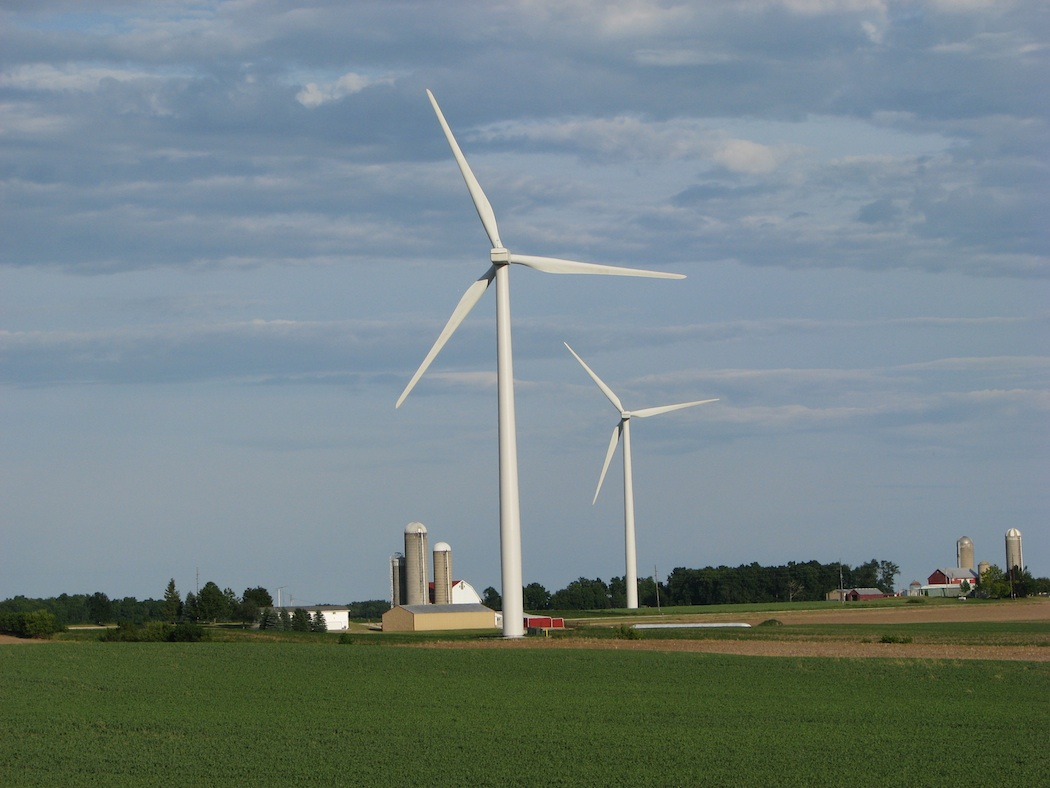
\includegraphics[height=2.5in]{files/21206}}
\hfill 
\subfigure[Aerial view of the National Wind Technology Center. 
 (Photo by Dennis Schroeder / NREL)\label{fig:20018}]
 {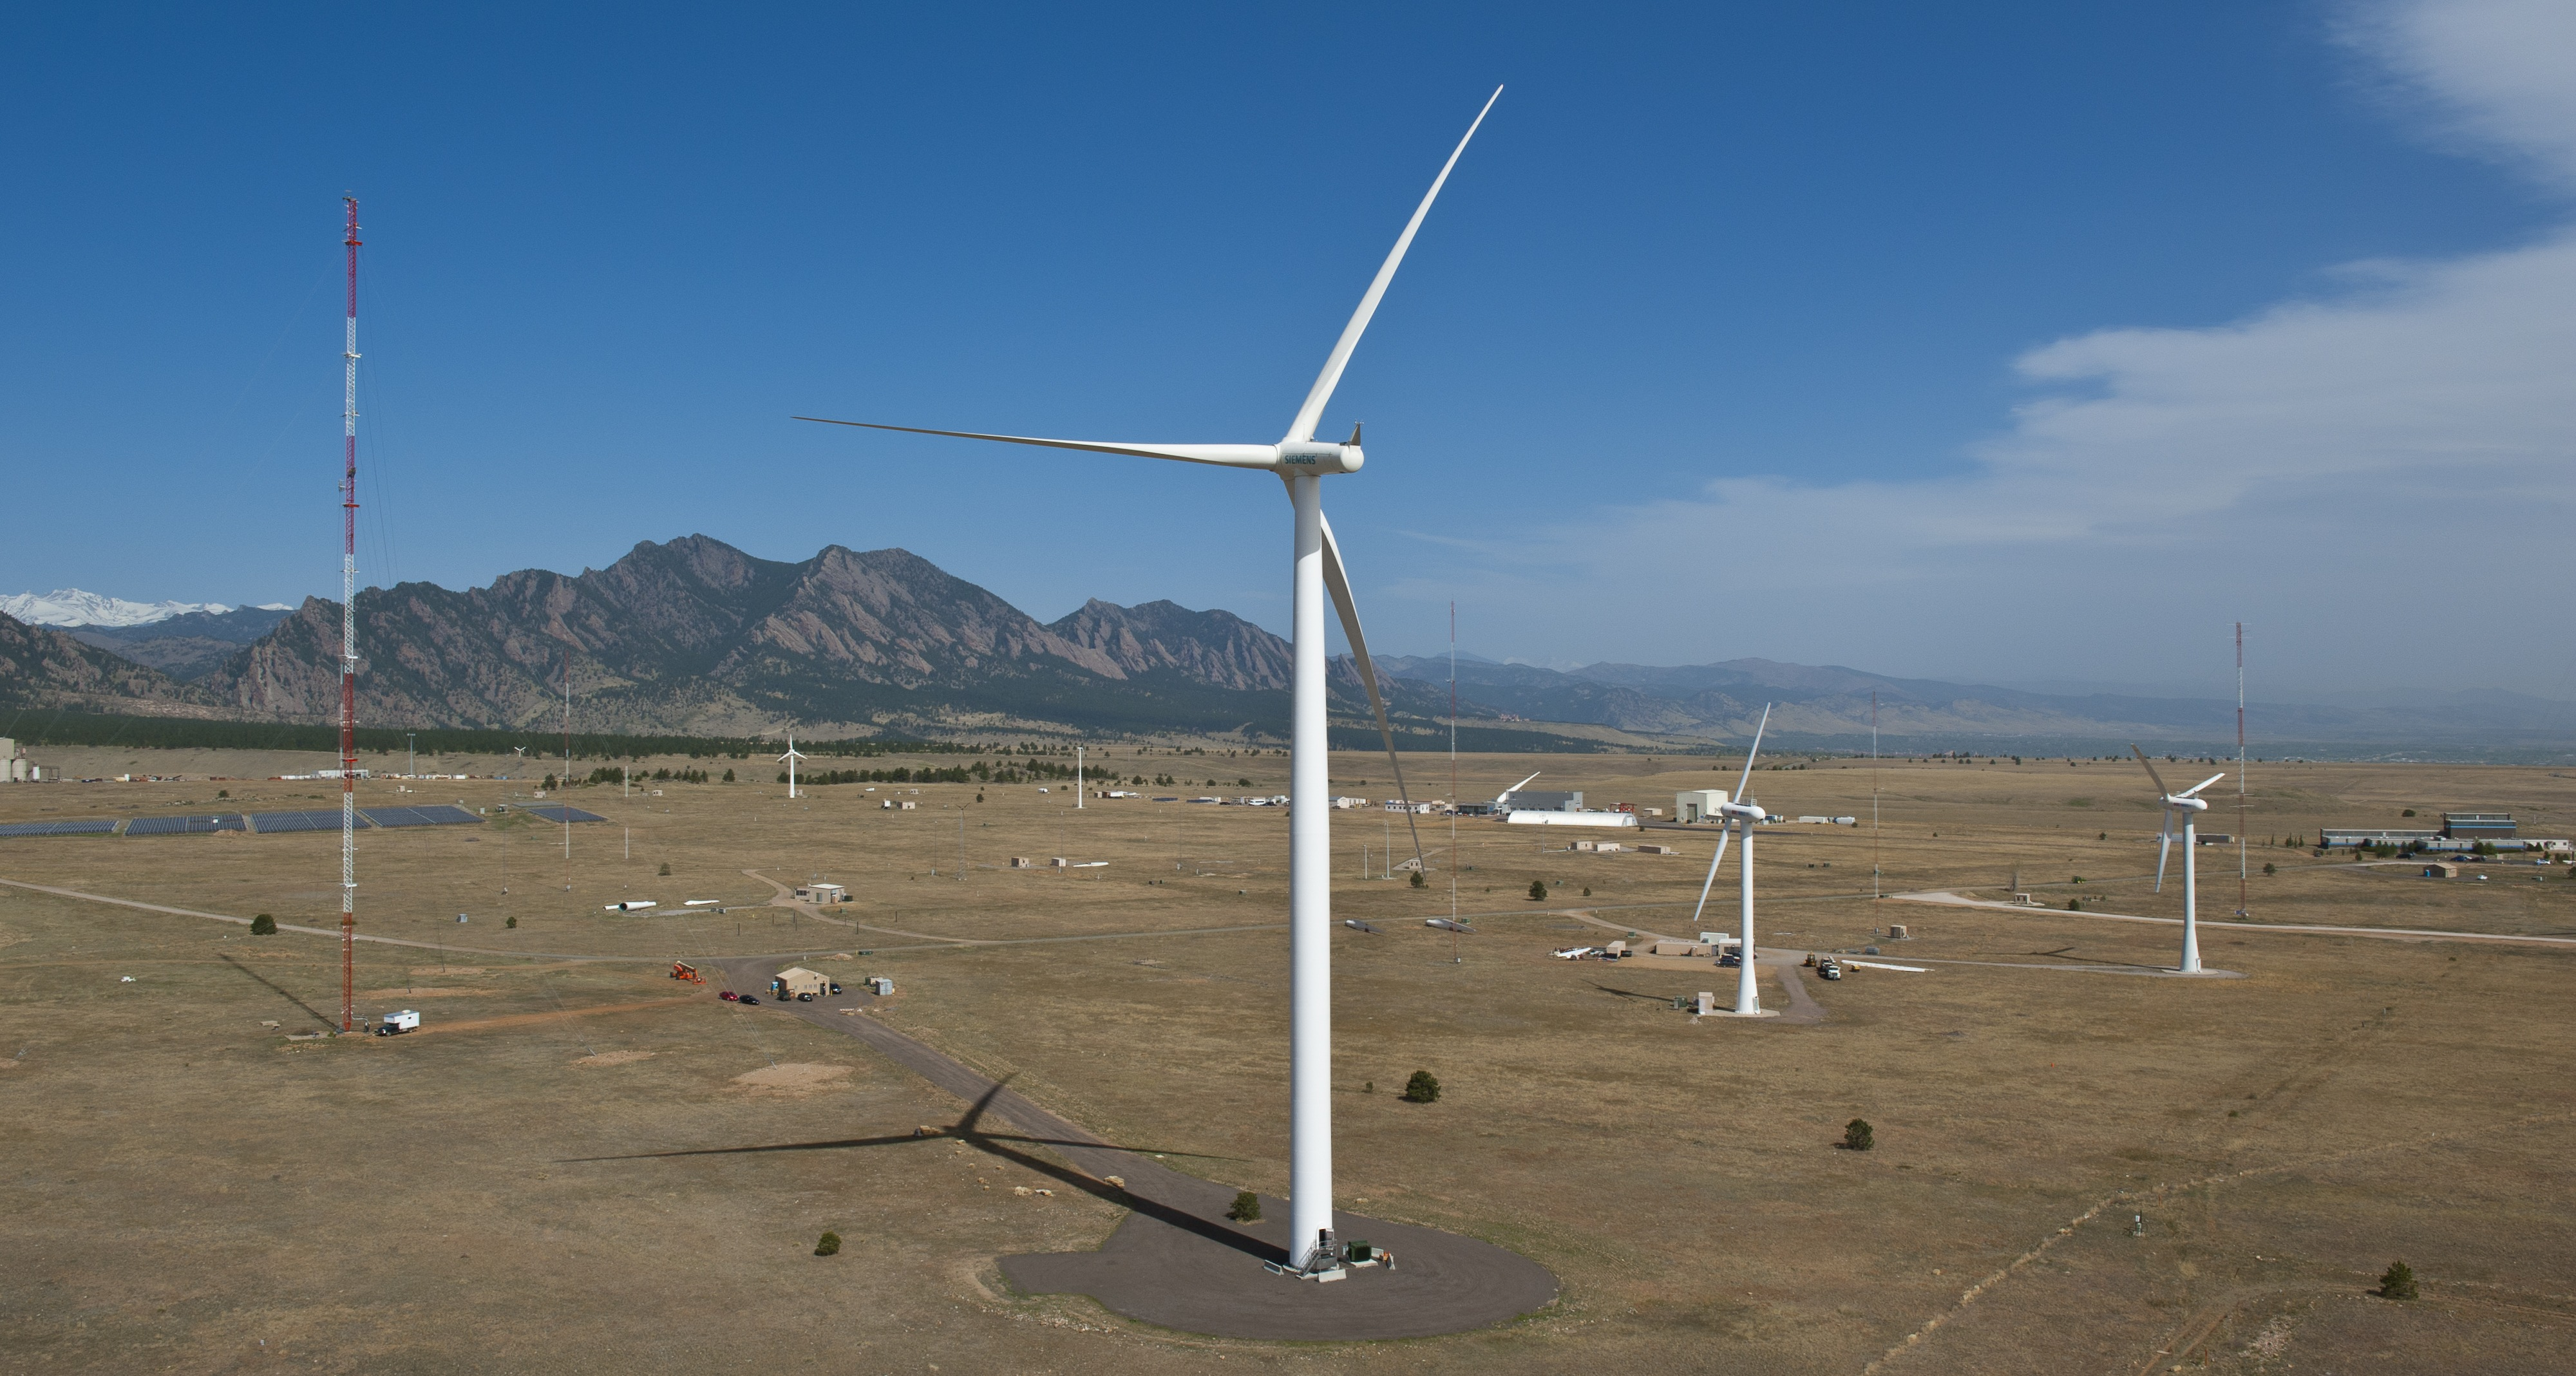
\includegraphics[height=2.5in]{files/20018}}
\hfill
\caption{NREL images}\label{fig:NRELimages}
\end{figure}
\end{verbatim}
 
\begin{figure*}[htp]
\centering
\hfill
\subfigure[Wind turbines at the Forward Wind Energy Center in Fond du Lac and Dodge Counties, Wisconsin. (Photo by Ruth Baranowski / NREL)\label{fig:21206}]{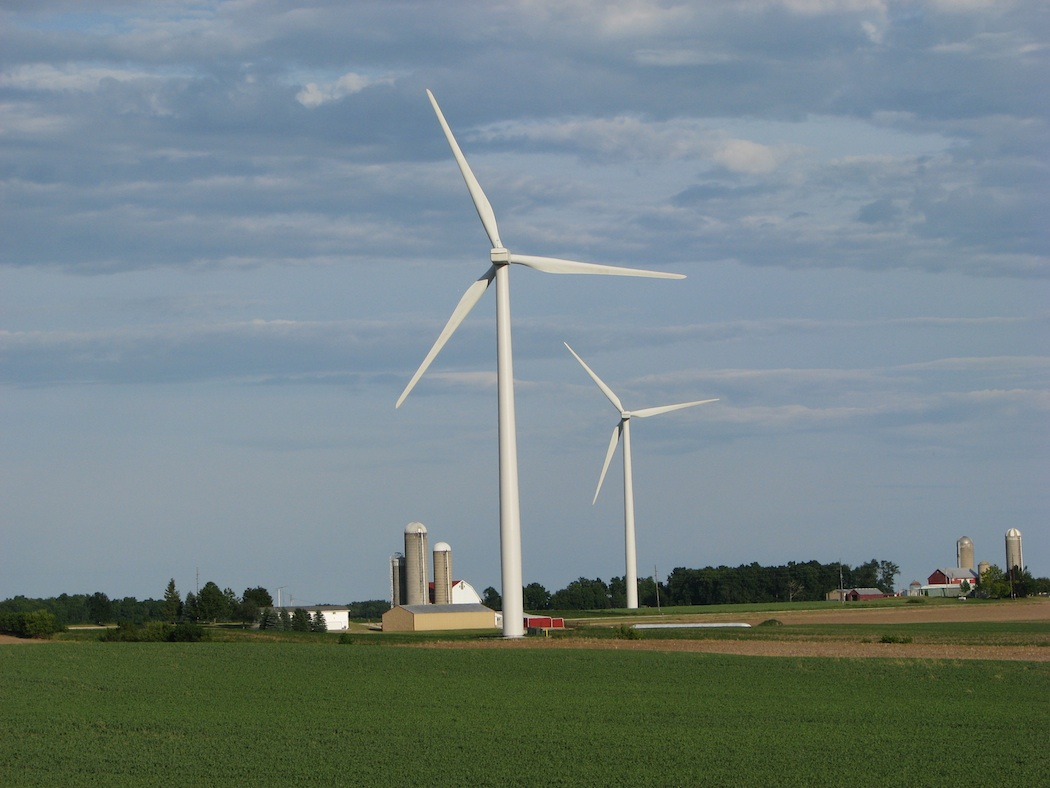
\includegraphics[height=2.5in]{files/21206}}
~ %add desired spacing between images, e. g. ~, \quad, \qquad etc. (or a blank line to force the subfigure onto a new line)
\hfill
\subfigure[Aerial view of the National Wind Technology Center. (Photo by Dennis Schroeder / NREL)\label{fig:20018}]{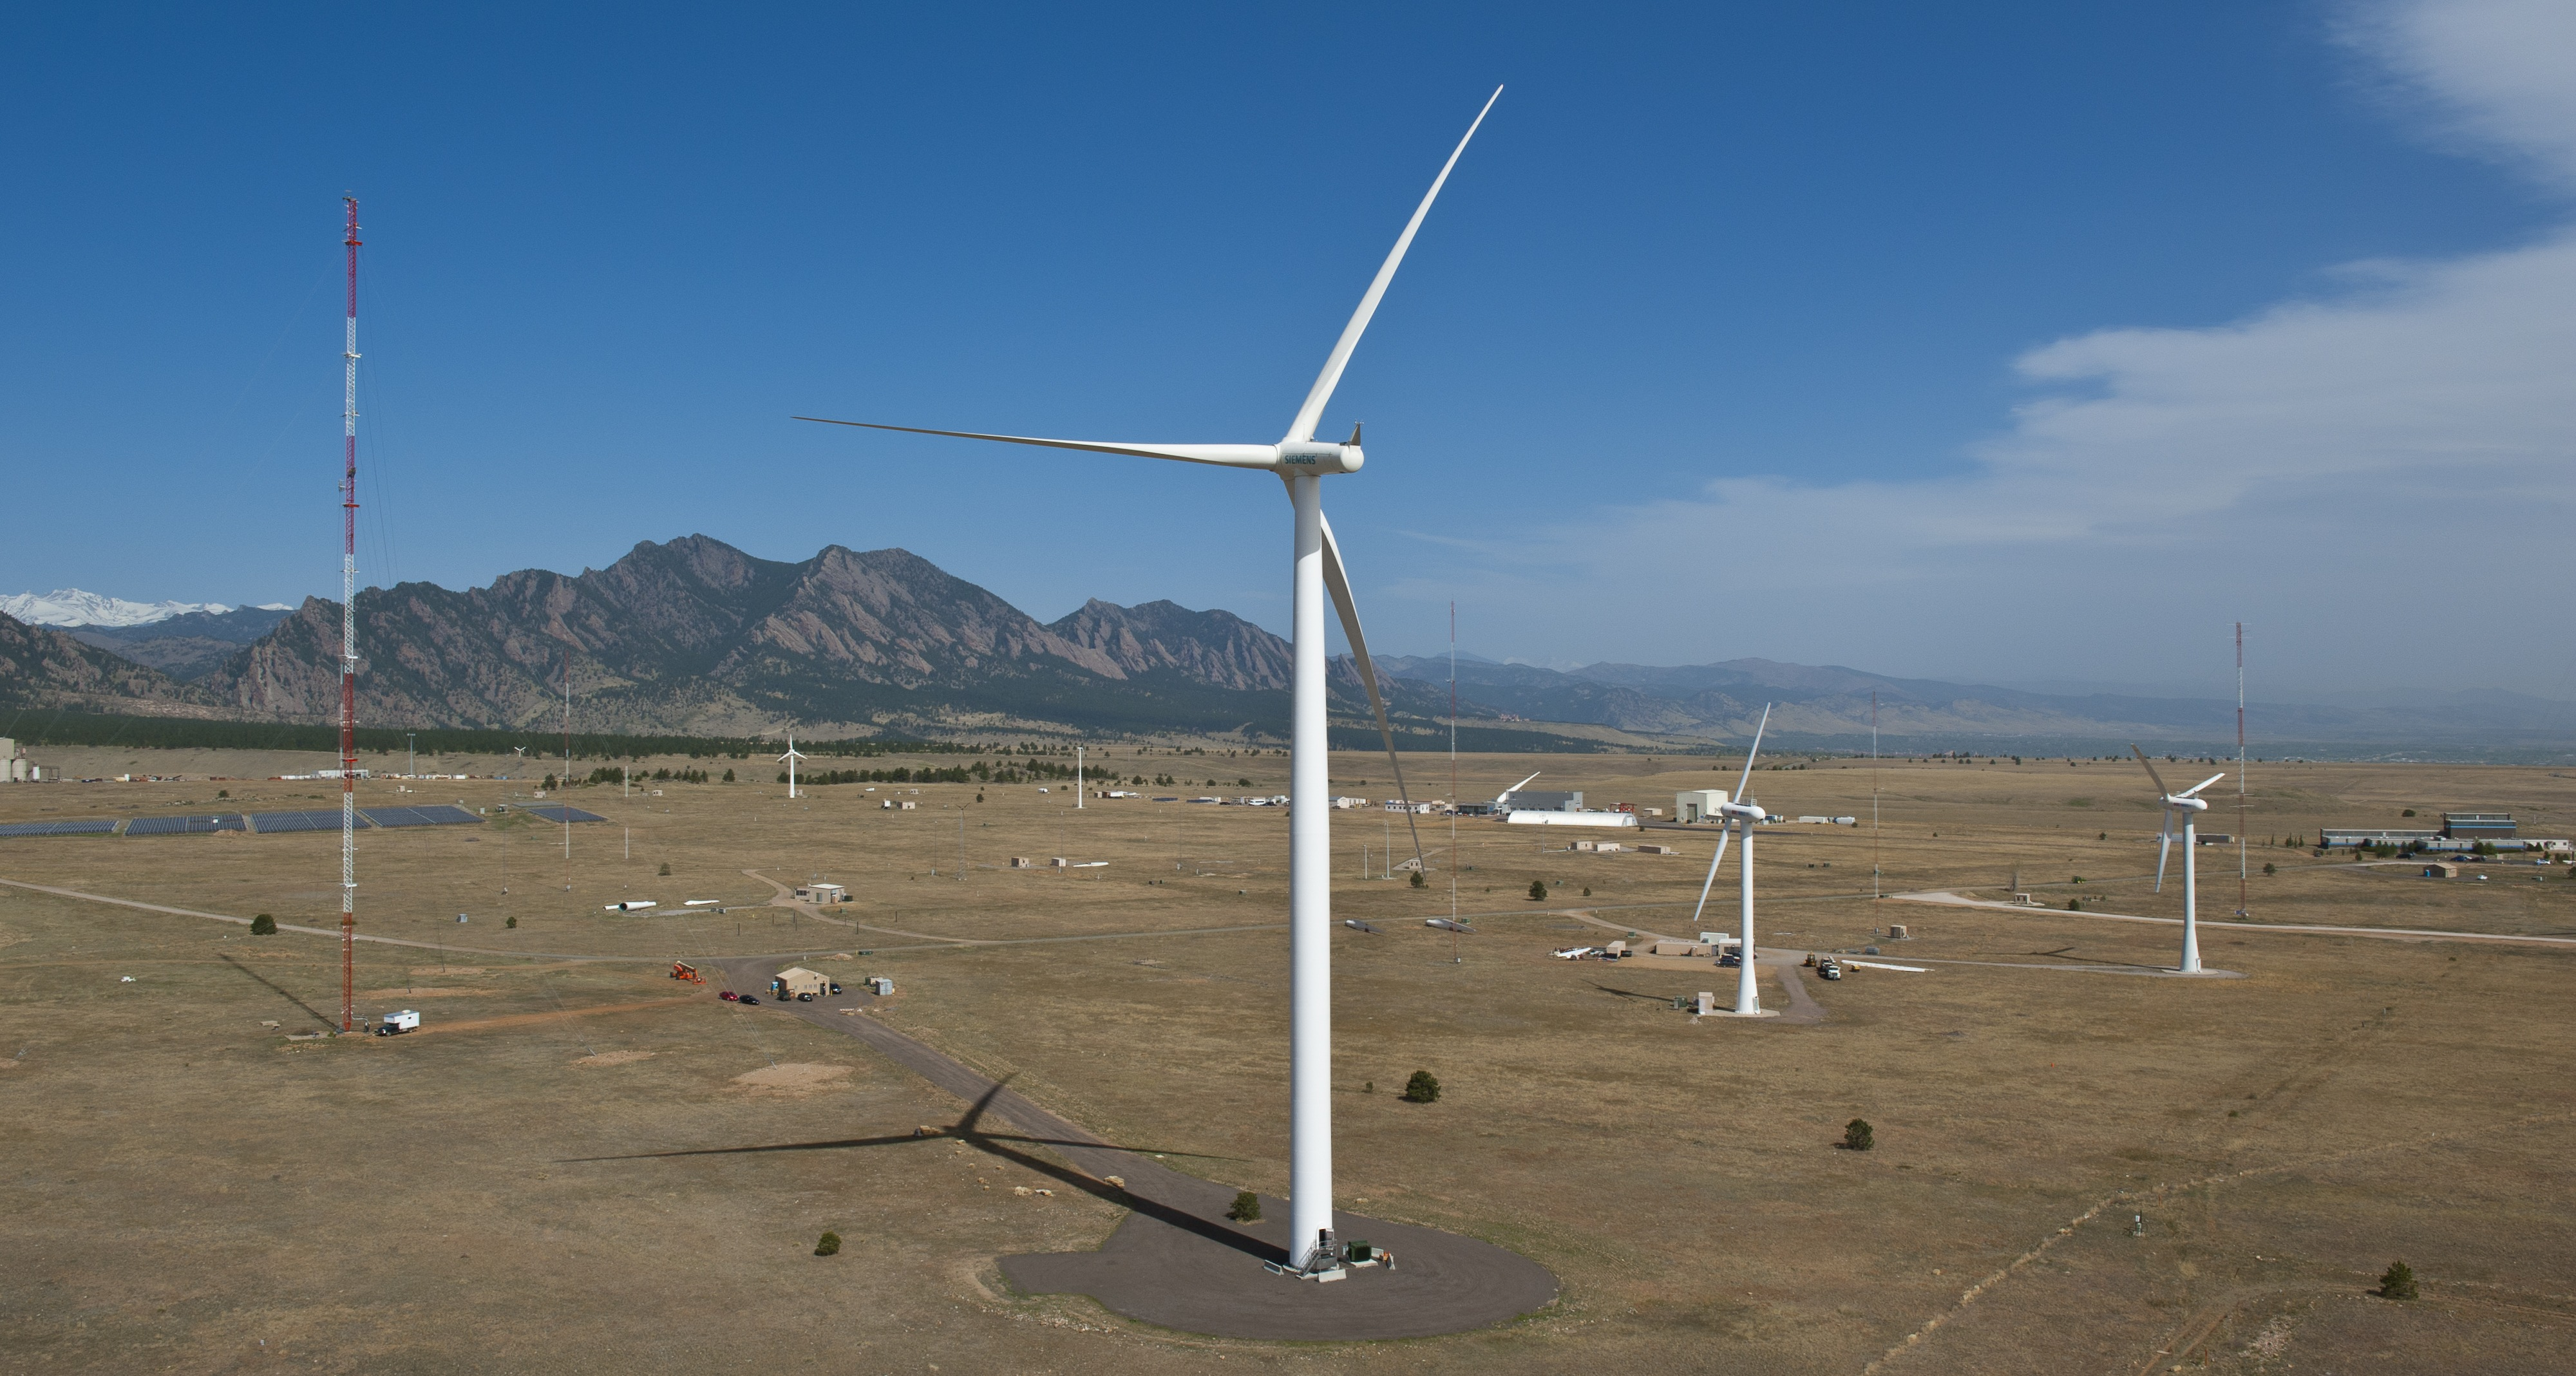
\includegraphics[height=2.5in]{files/20018}}
\hfill
\caption{NREL images}\label{fig:NRELimages}
\end{figure*}

If a subfigure is split over two lines using \verb+\\+, make sure those symbols are on their own line.

\section{Lists}

To make lists with automatic numbering, use the \texttt{enumerate} environment:

\begin{enumerate}
\item Like this,
\item and like this.
\end{enumerate}
\dots or bullet points \dots
\begin{itemize}
\item Like this,
\item and like this.
\end{itemize}

\section{Computer code}
The \texttt{lstlisting} package has been loaded.

\section{Creating a file structure}
\label{sec:FileStructure}
Use the \texttt{input} command to import other files into your main file. For example, each of the chapters in this report could be in separate files, called \emph{NRELRequirements} (Chapter 1), \emph{LatexAtNREL} (Chapter 2), and so-on. 

\begin{verbatim}
...
% content
\input{NRELRequirements}
\input{LatexAtNREL}
\chapter{Some LaTeX examples}
This chapter includes examples of how to do common tasks using LaTeX{}. Although most users will be familiar with these commands and environments, these serve as a) a test of the class file and conversion process, and b) examples that are known to work with the class and conversion process. So, when all else fails, users can copy these examples and tailor them to their particular case.

\section{Headings}
LaTeX{} allows a very simple definition of the document's structure. This document has the following structure:
\begin{itemize}
\item Chapter 1: what is LaTeX?
\begin{itemize}
\item Section 1: Headings
\item Section 2: Floats
\item Section 3: Mathematics
\item Section 4: Lists
\end{itemize}
\item etc. \ldots
\end{itemize}

\subsection{Chapter}
To define a new chapter, simply write \verb+\chapter{What is LaTeX?}+.

To use chapters, pass the \texttt{memoir}, \texttt{book}, or \texttt{report} option to \emph{nrel.cls} (see Section \ref{sec:nrel.cls.options}).

\subsection{Sections}
If Chapters are the highest level headings in a document, sections come next, followed by subsections. Although there don't have to be chapters in a document, a LaTeX document does need to have Sections.

So: 

\begin{verbatim}
\section{Headings}
LaTeX{} allows a very simple definition of the document's structure. 
This document has the following structure:
...
\subsection{Chapter}

\end{verbatim}

\section{Body text}
Body text does not need to be specially identified in LaTeX{}. Non-printing comments are identified in the source document(s) using the \% symbol.

\section{Mathematics}

LaTeX is great at typesetting mathematics. The following example is taken from the \href{www.writelatex.com}{www.writelatex.com} website:

\begin{quote}
Making inline equations is easy. Let $X_1, X_2, \ldots, X_n$ be a sequence of independent and identically distributed random variables with $\textrm{E}[X_i] = \mu$ and $\textrm{Var}[X_i] = \sigma^2 < \infty$, and let
$$S_n = \frac{X_1 + X_2 + \cdots + X_n}{n}
 = \frac{1}{n}\sum_{i}^{n} X_i$$
denote their mean. Then as $n$ approaches infinity, the random variables $\sqrt{n}(S_n - \mu)$ converge in distribution to a normal $\mathcal{N}(0, \sigma^2)$.
\end{quote}

Alternatively, if numbered equations are required, use the \texttt{equation} environment. For example:

\begin{verbatim}
\begin{equation}
y = mx +c \textrm{.}
\label{eqn:line}
\end{equation}
\end{verbatim}

would give:

\begin{equation}
y = mx+c \textrm{.}
\label{eqn:line}
\end{equation}

\section{Cross references}
Use labels and references to refer back and forth to figures, equations, tables and sections. For example, \verb+Eqn. \ref{eqn:line}+ gives a reference to Eqn. \ref{eqn:line}.

\section{Floats}
Floats are images, tables or other pieces of the document that are free to move to the best place in the document for them. Literally, they `float'. The two most common floats are the tabular environment (for tables) and the figure environment for figures.

\subsection{Tables}
Use the \texttt{tabular} environment to produce basic tables. Table~\ref{tab:widgets} is produced using this code: 

\begin{verbatim}
\begin{table}[!h]
\centering
\caption{An example table.}\label{tab:widgets}
\begin{tabular}{lr}
Item & Quantity \\\hline
Widgets & 42 \\
Gadgets & 13
\end{tabular}
\end{table}
\end{verbatim}

\begin{table}[!h]
\centering
\caption{An example table.}\label{tab:widgets}
\begin{tabular}{lr}
Item & Quantity \\\hline
Widgets & 42 \\
Gadgets & 13
\end{tabular}
\end{table}

Resist the temptation to stop table rows early. If all of the delimiters  (\&) are included in each row, the table will be complete and will better translate to RTF later.

\subsection{Figures}
To include a figure in a document, use the \texttt{figure} environment and the \texttt{includegraphics} command.

\begin{verbatim}
\begin{figure}
\includegraphics[width=\textwidth]{figure's-file-name}
\caption{Caption goes here.}\label{fig:figuresLabel}
\end{figure}
\end{verbatim}

\subsection{Subfigures}
Subfigures are implemented using the \texttt{subfig} package. Although this package is deprecated (apparently \texttt{subcaption} is now the preferred package), it plays fairly nicely with \texttt{latex2rtf} so will be used for the foreseeable future. 

The \texttt{label}s in the example below allow us to make references using the \texttt{ref} command, both to the overall figure (Figure \ref{fig:NRELimages}) and the subfigures (Figures \ref{fig:21206} and \ref{fig:20018}) directly. Unfortunately, \texttt{latex2rtf} does not allow multiple \texttt{label}s in a Figure environment, and so only the first label will be kept: therefore, it's best to just use a single label in any one \texttt{figure} environment.

\begin{verbatim}
\begin{figure}
\centering
\hfill
\subfigure[Wind turbines at the Forward Wind Energy Center in Fond du Lac 
 and Dodge Counties, Wisconsin. (Photo by Ruth Baranowski / NREL)
 \label{fig:21206}]{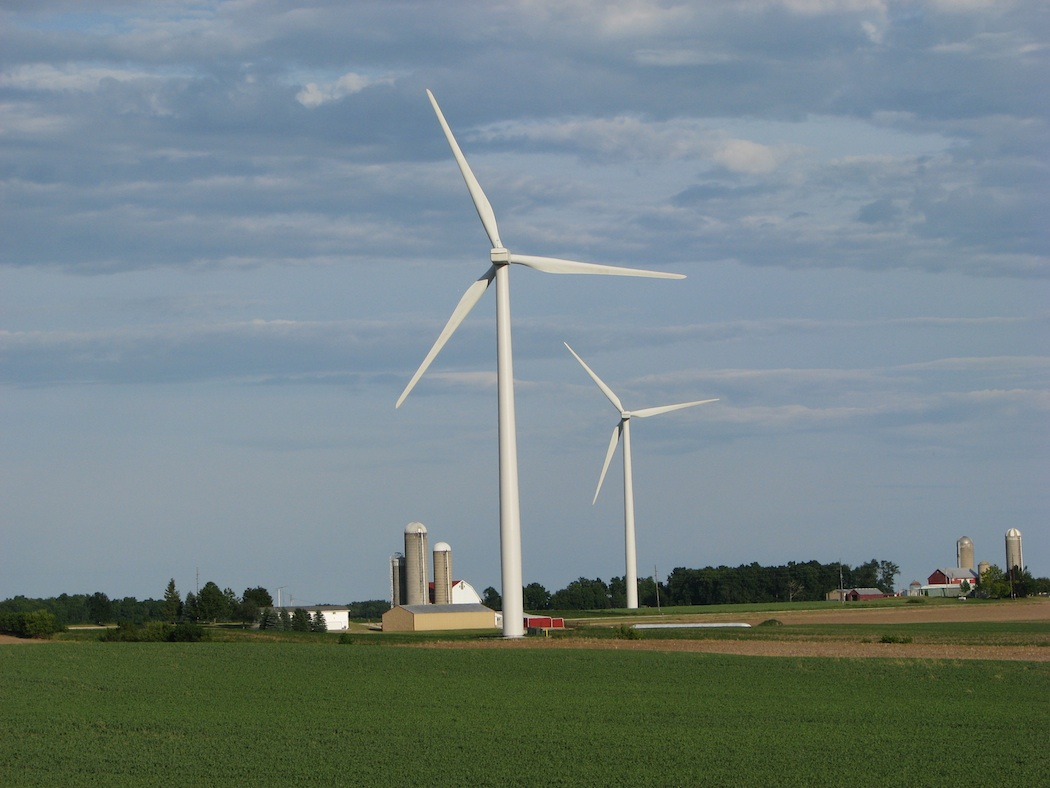
\includegraphics[height=2.5in]{files/21206}}
\hfill 
\subfigure[Aerial view of the National Wind Technology Center. 
 (Photo by Dennis Schroeder / NREL)\label{fig:20018}]
 {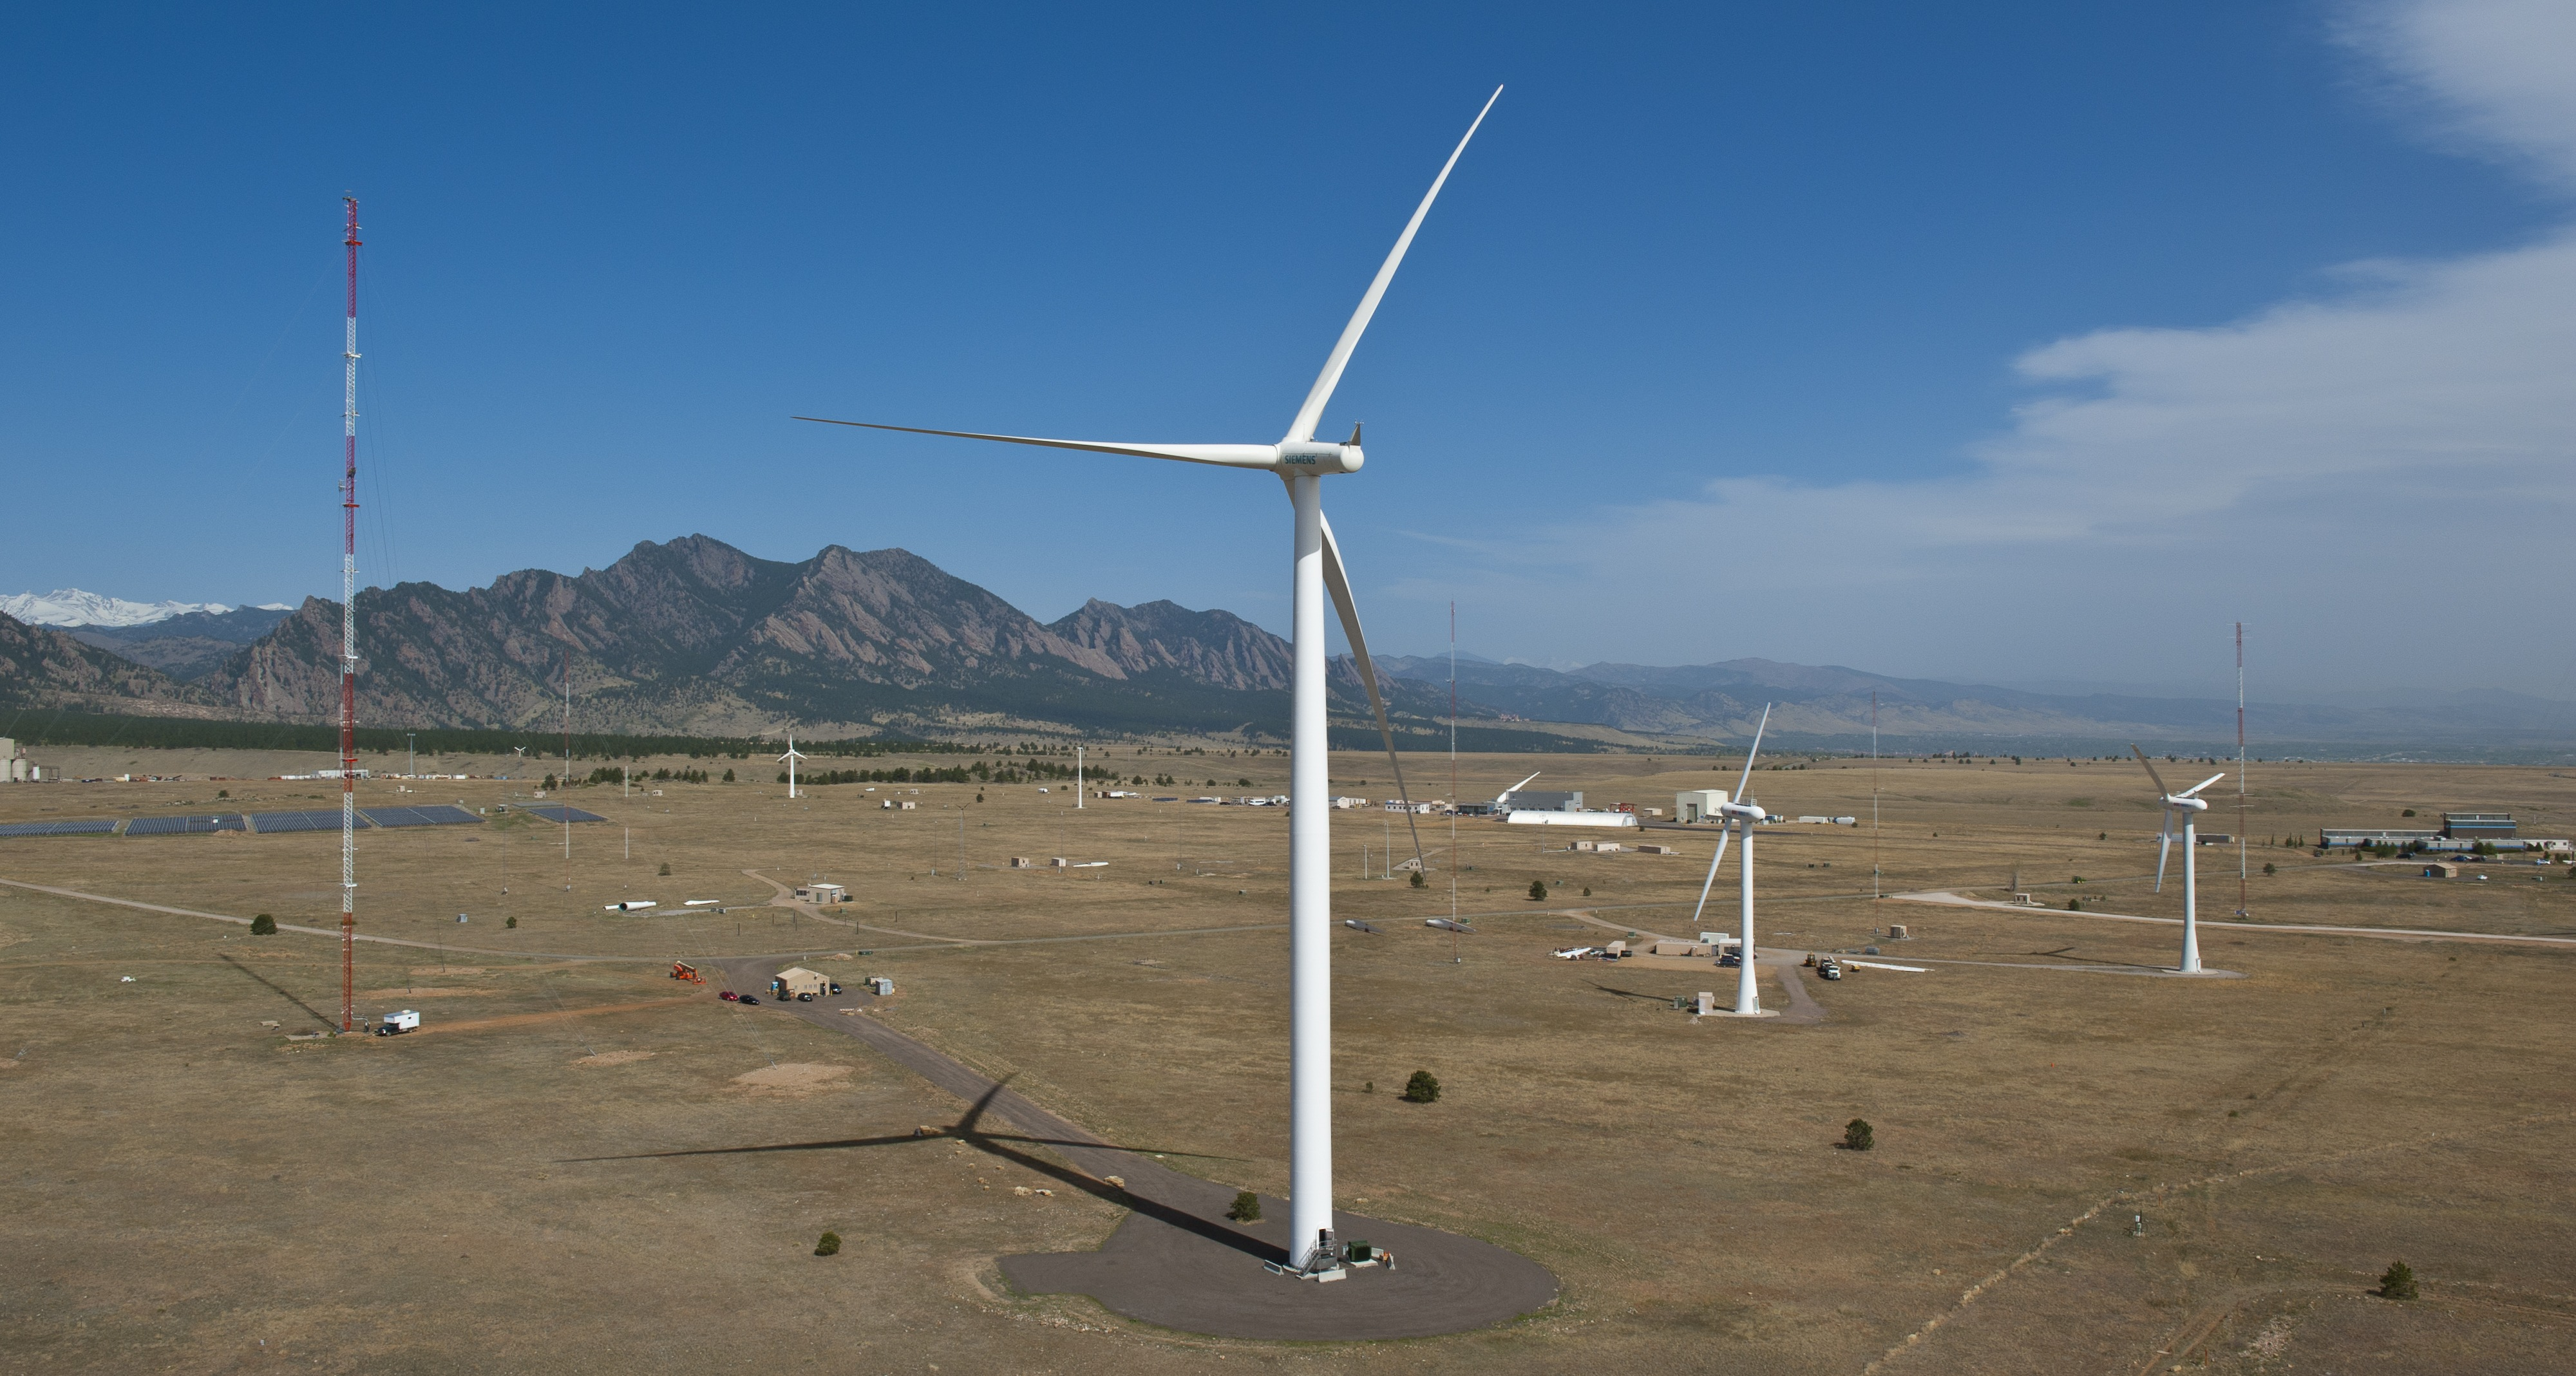
\includegraphics[height=2.5in]{files/20018}}
\hfill
\caption{NREL images}\label{fig:NRELimages}
\end{figure}
\end{verbatim}
 
\begin{figure*}[htp]
\centering
\hfill
\subfigure[Wind turbines at the Forward Wind Energy Center in Fond du Lac and Dodge Counties, Wisconsin. (Photo by Ruth Baranowski / NREL)\label{fig:21206}]{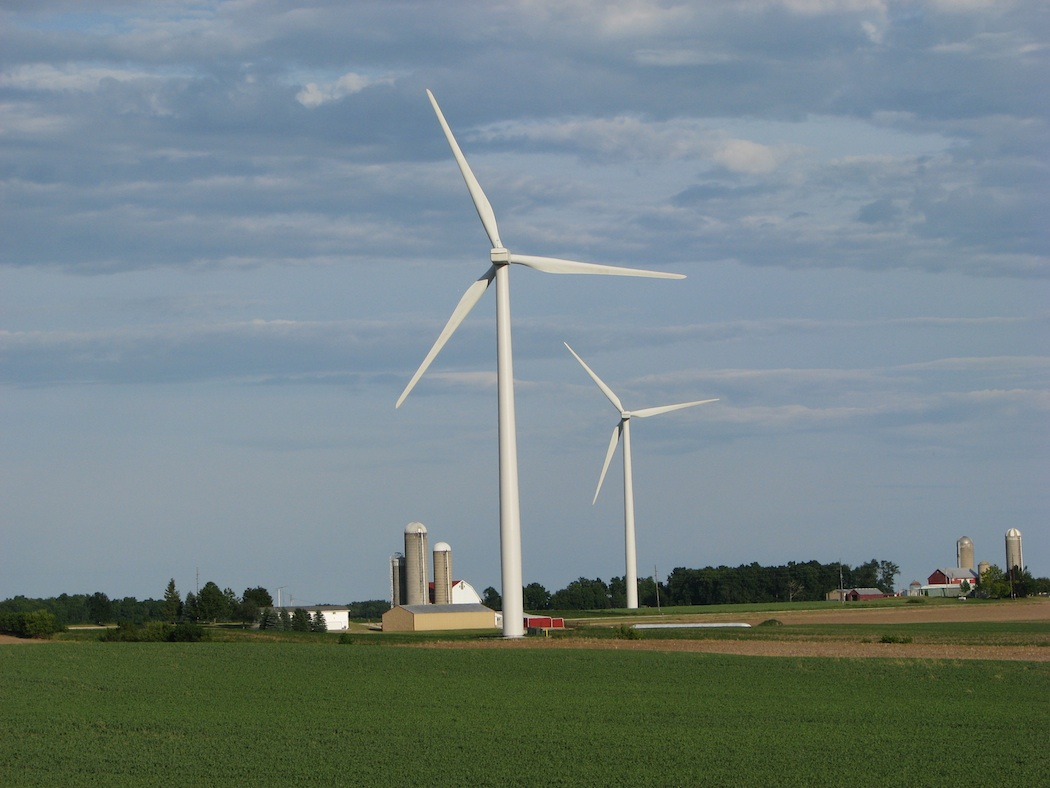
\includegraphics[height=2.5in]{files/21206}}
~ %add desired spacing between images, e. g. ~, \quad, \qquad etc. (or a blank line to force the subfigure onto a new line)
\hfill
\subfigure[Aerial view of the National Wind Technology Center. (Photo by Dennis Schroeder / NREL)\label{fig:20018}]{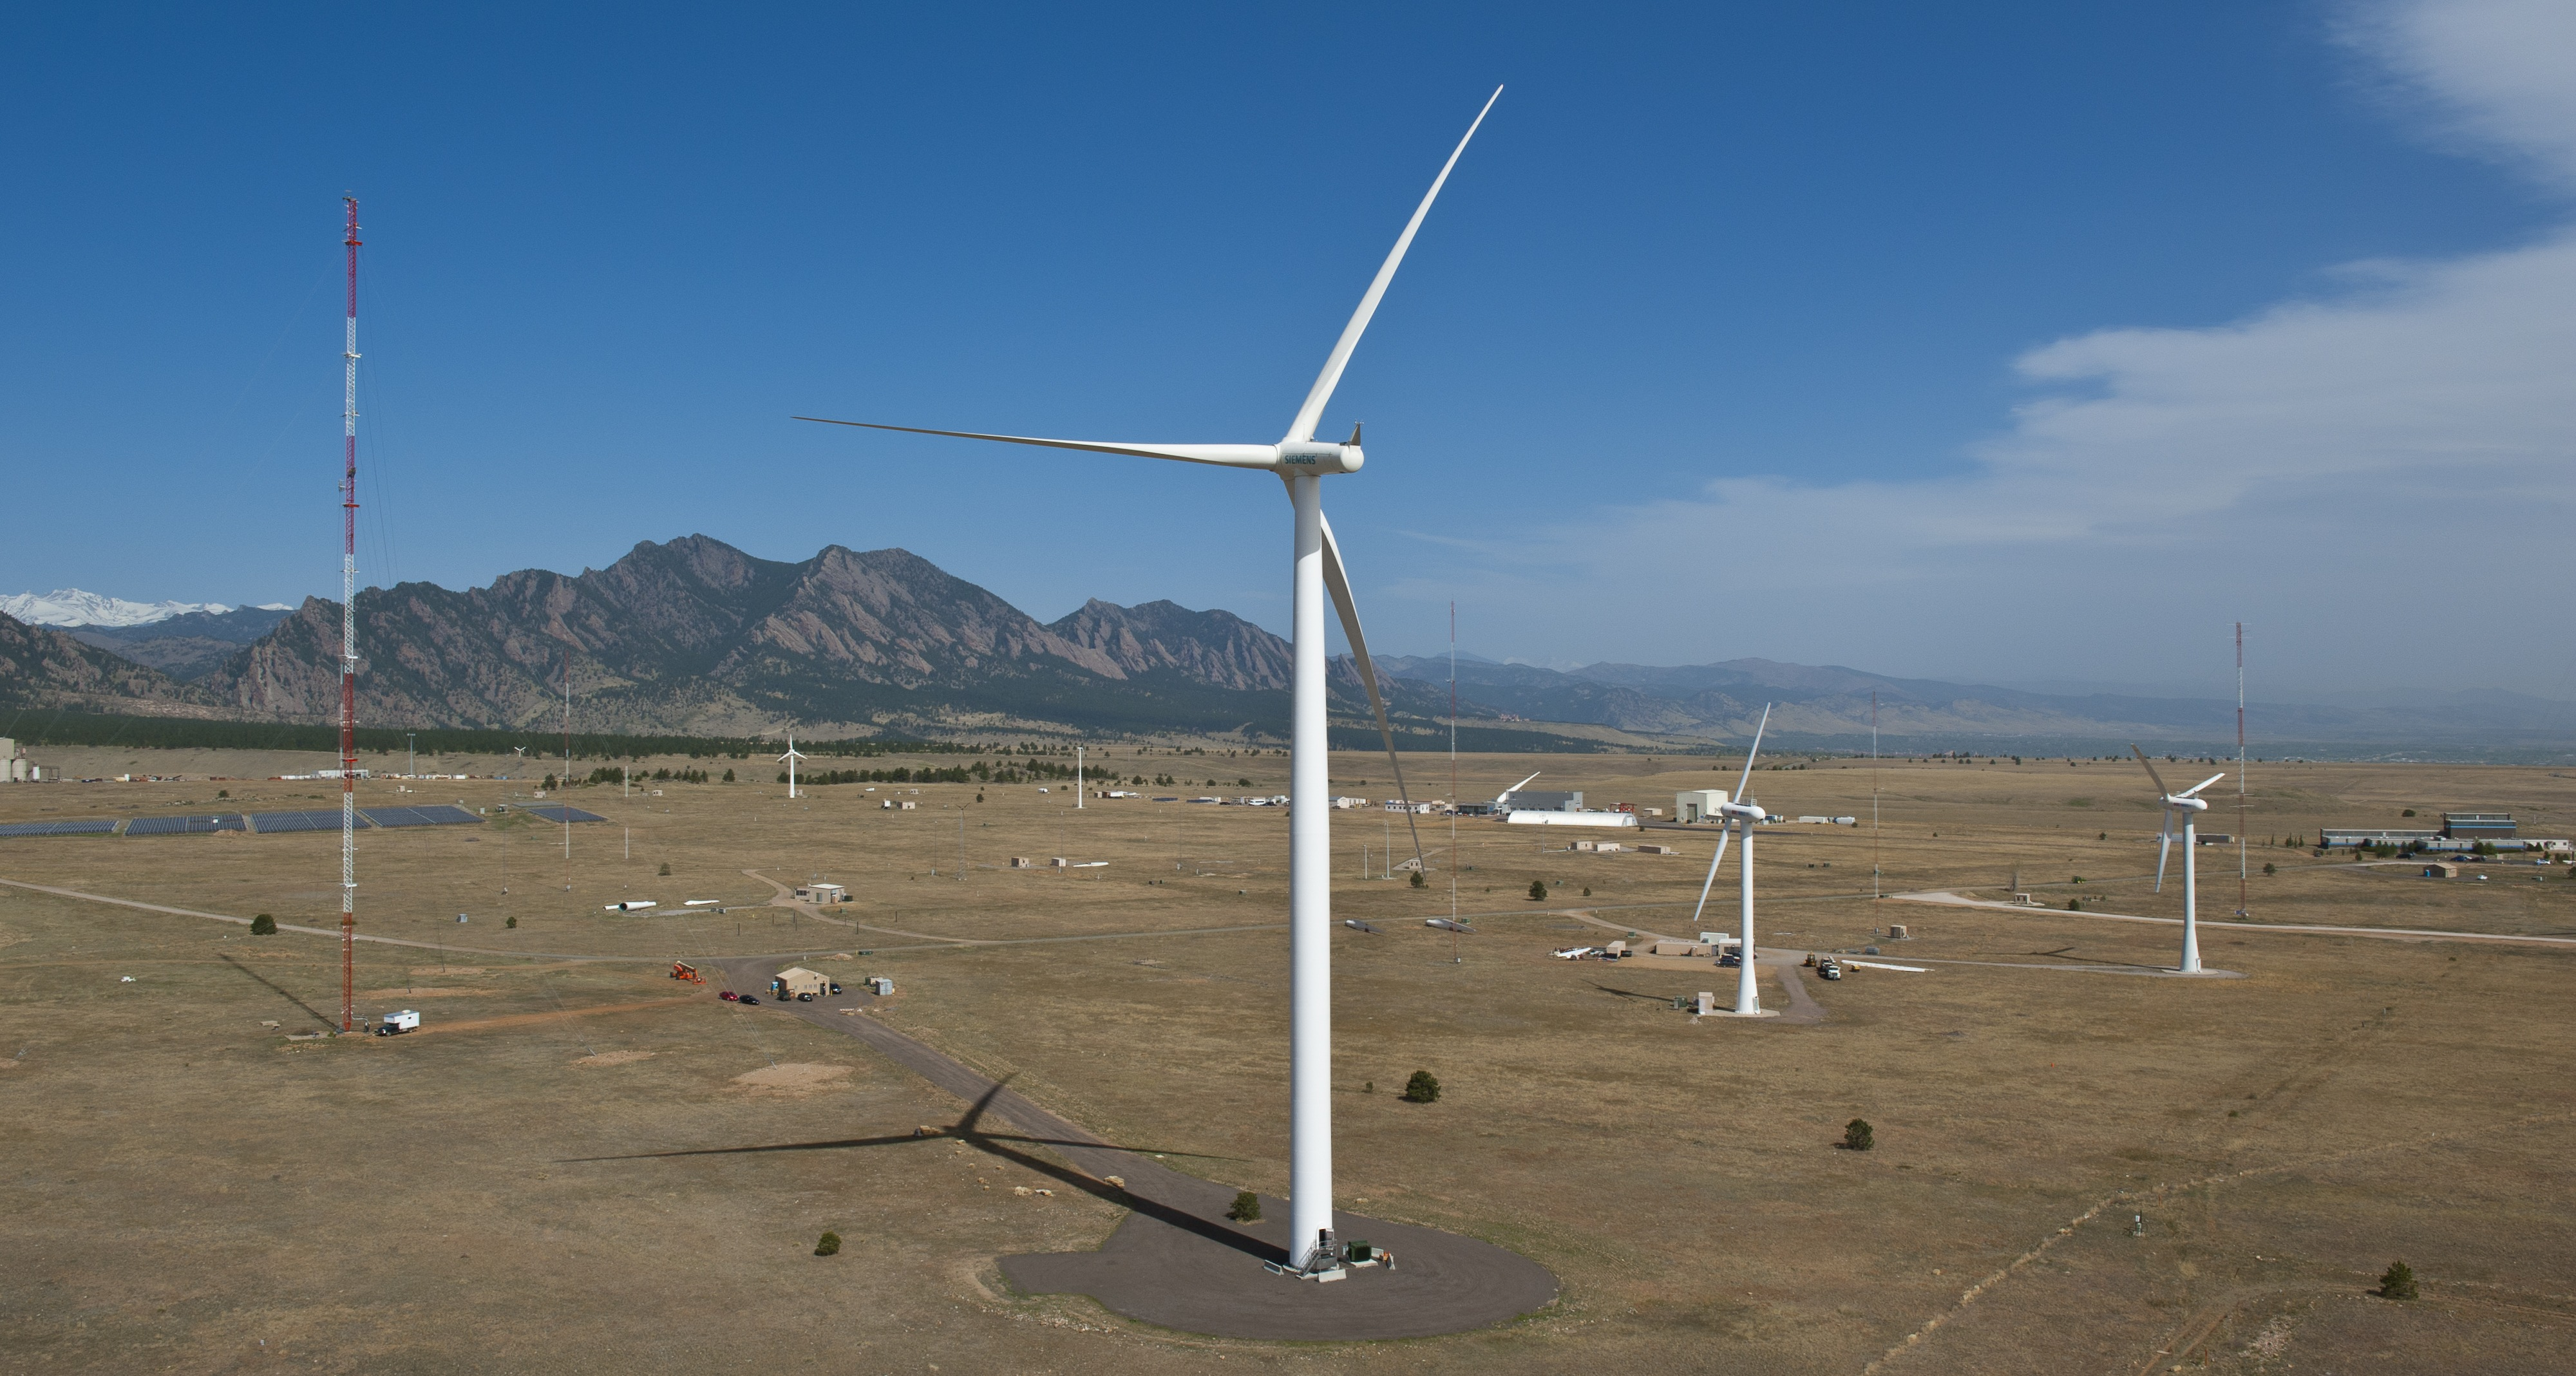
\includegraphics[height=2.5in]{files/20018}}
\hfill
\caption{NREL images}\label{fig:NRELimages}
\end{figure*}

If a subfigure is split over two lines using \verb+\\+, make sure those symbols are on their own line.

\section{Lists}

To make lists with automatic numbering, use the \texttt{enumerate} environment:

\begin{enumerate}
\item Like this,
\item and like this.
\end{enumerate}
\dots or bullet points \dots
\begin{itemize}
\item Like this,
\item and like this.
\end{itemize}

\section{Computer code}
The \texttt{lstlisting} package has been loaded.

\section{Creating a file structure}
\label{sec:FileStructure}
Use the \texttt{input} command to import other files into your main file. For example, each of the chapters in this report could be in separate files, called \emph{NRELRequirements} (Chapter 1), \emph{LatexAtNREL} (Chapter 2), and so-on. 

\begin{verbatim}
...
% content
\input{NRELRequirements}
\input{LatexAtNREL}
\chapter{Some LaTeX examples}
This chapter includes examples of how to do common tasks using LaTeX{}. Although most users will be familiar with these commands and environments, these serve as a) a test of the class file and conversion process, and b) examples that are known to work with the class and conversion process. So, when all else fails, users can copy these examples and tailor them to their particular case.

\section{Headings}
LaTeX{} allows a very simple definition of the document's structure. This document has the following structure:
\begin{itemize}
\item Chapter 1: what is LaTeX?
\begin{itemize}
\item Section 1: Headings
\item Section 2: Floats
\item Section 3: Mathematics
\item Section 4: Lists
\end{itemize}
\item etc. \ldots
\end{itemize}

\subsection{Chapter}
To define a new chapter, simply write \verb+\chapter{What is LaTeX?}+.

To use chapters, pass the \texttt{memoir}, \texttt{book}, or \texttt{report} option to \emph{nrel.cls} (see Section \ref{sec:nrel.cls.options}).

\subsection{Sections}
If Chapters are the highest level headings in a document, sections come next, followed by subsections. Although there don't have to be chapters in a document, a LaTeX document does need to have Sections.

So: 

\begin{verbatim}
\section{Headings}
LaTeX{} allows a very simple definition of the document's structure. 
This document has the following structure:
...
\subsection{Chapter}

\end{verbatim}

\section{Body text}
Body text does not need to be specially identified in LaTeX{}. Non-printing comments are identified in the source document(s) using the \% symbol.

\section{Mathematics}

LaTeX is great at typesetting mathematics. The following example is taken from the \href{www.writelatex.com}{www.writelatex.com} website:

\begin{quote}
Making inline equations is easy. Let $X_1, X_2, \ldots, X_n$ be a sequence of independent and identically distributed random variables with $\textrm{E}[X_i] = \mu$ and $\textrm{Var}[X_i] = \sigma^2 < \infty$, and let
$$S_n = \frac{X_1 + X_2 + \cdots + X_n}{n}
 = \frac{1}{n}\sum_{i}^{n} X_i$$
denote their mean. Then as $n$ approaches infinity, the random variables $\sqrt{n}(S_n - \mu)$ converge in distribution to a normal $\mathcal{N}(0, \sigma^2)$.
\end{quote}

Alternatively, if numbered equations are required, use the \texttt{equation} environment. For example:

\begin{verbatim}
\begin{equation}
y = mx +c \textrm{.}
\label{eqn:line}
\end{equation}
\end{verbatim}

would give:

\begin{equation}
y = mx+c \textrm{.}
\label{eqn:line}
\end{equation}

\section{Cross references}
Use labels and references to refer back and forth to figures, equations, tables and sections. For example, \verb+Eqn. \ref{eqn:line}+ gives a reference to Eqn. \ref{eqn:line}.

\section{Floats}
Floats are images, tables or other pieces of the document that are free to move to the best place in the document for them. Literally, they `float'. The two most common floats are the tabular environment (for tables) and the figure environment for figures.

\subsection{Tables}
Use the \texttt{tabular} environment to produce basic tables. Table~\ref{tab:widgets} is produced using this code: 

\begin{verbatim}
\begin{table}[!h]
\centering
\caption{An example table.}\label{tab:widgets}
\begin{tabular}{lr}
Item & Quantity \\\hline
Widgets & 42 \\
Gadgets & 13
\end{tabular}
\end{table}
\end{verbatim}

\begin{table}[!h]
\centering
\caption{An example table.}\label{tab:widgets}
\begin{tabular}{lr}
Item & Quantity \\\hline
Widgets & 42 \\
Gadgets & 13
\end{tabular}
\end{table}

Resist the temptation to stop table rows early. If all of the delimiters  (\&) are included in each row, the table will be complete and will better translate to RTF later.

\subsection{Figures}
To include a figure in a document, use the \texttt{figure} environment and the \texttt{includegraphics} command.

\begin{verbatim}
\begin{figure}
\includegraphics[width=\textwidth]{figure's-file-name}
\caption{Caption goes here.}\label{fig:figuresLabel}
\end{figure}
\end{verbatim}

\subsection{Subfigures}
Subfigures are implemented using the \texttt{subfig} package. Although this package is deprecated (apparently \texttt{subcaption} is now the preferred package), it plays fairly nicely with \texttt{latex2rtf} so will be used for the foreseeable future. 

The \texttt{label}s in the example below allow us to make references using the \texttt{ref} command, both to the overall figure (Figure \ref{fig:NRELimages}) and the subfigures (Figures \ref{fig:21206} and \ref{fig:20018}) directly. Unfortunately, \texttt{latex2rtf} does not allow multiple \texttt{label}s in a Figure environment, and so only the first label will be kept: therefore, it's best to just use a single label in any one \texttt{figure} environment.

\begin{verbatim}
\begin{figure}
\centering
\hfill
\subfigure[Wind turbines at the Forward Wind Energy Center in Fond du Lac 
 and Dodge Counties, Wisconsin. (Photo by Ruth Baranowski / NREL)
 \label{fig:21206}]{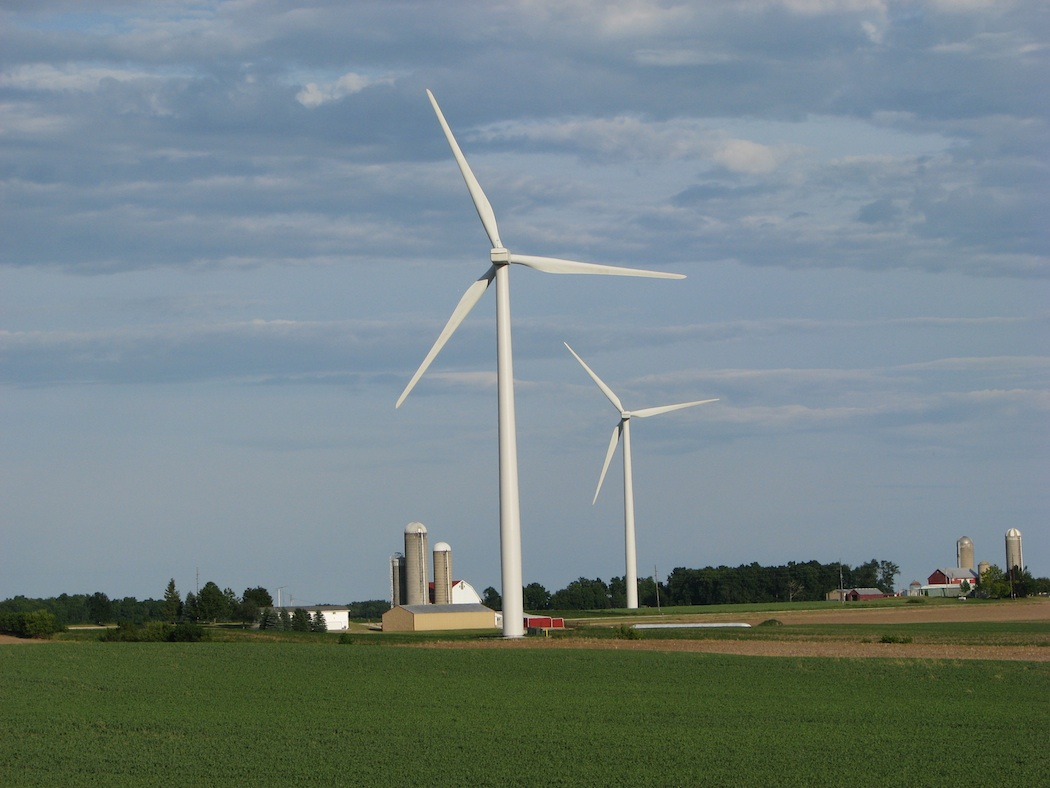
\includegraphics[height=2.5in]{files/21206}}
\hfill 
\subfigure[Aerial view of the National Wind Technology Center. 
 (Photo by Dennis Schroeder / NREL)\label{fig:20018}]
 {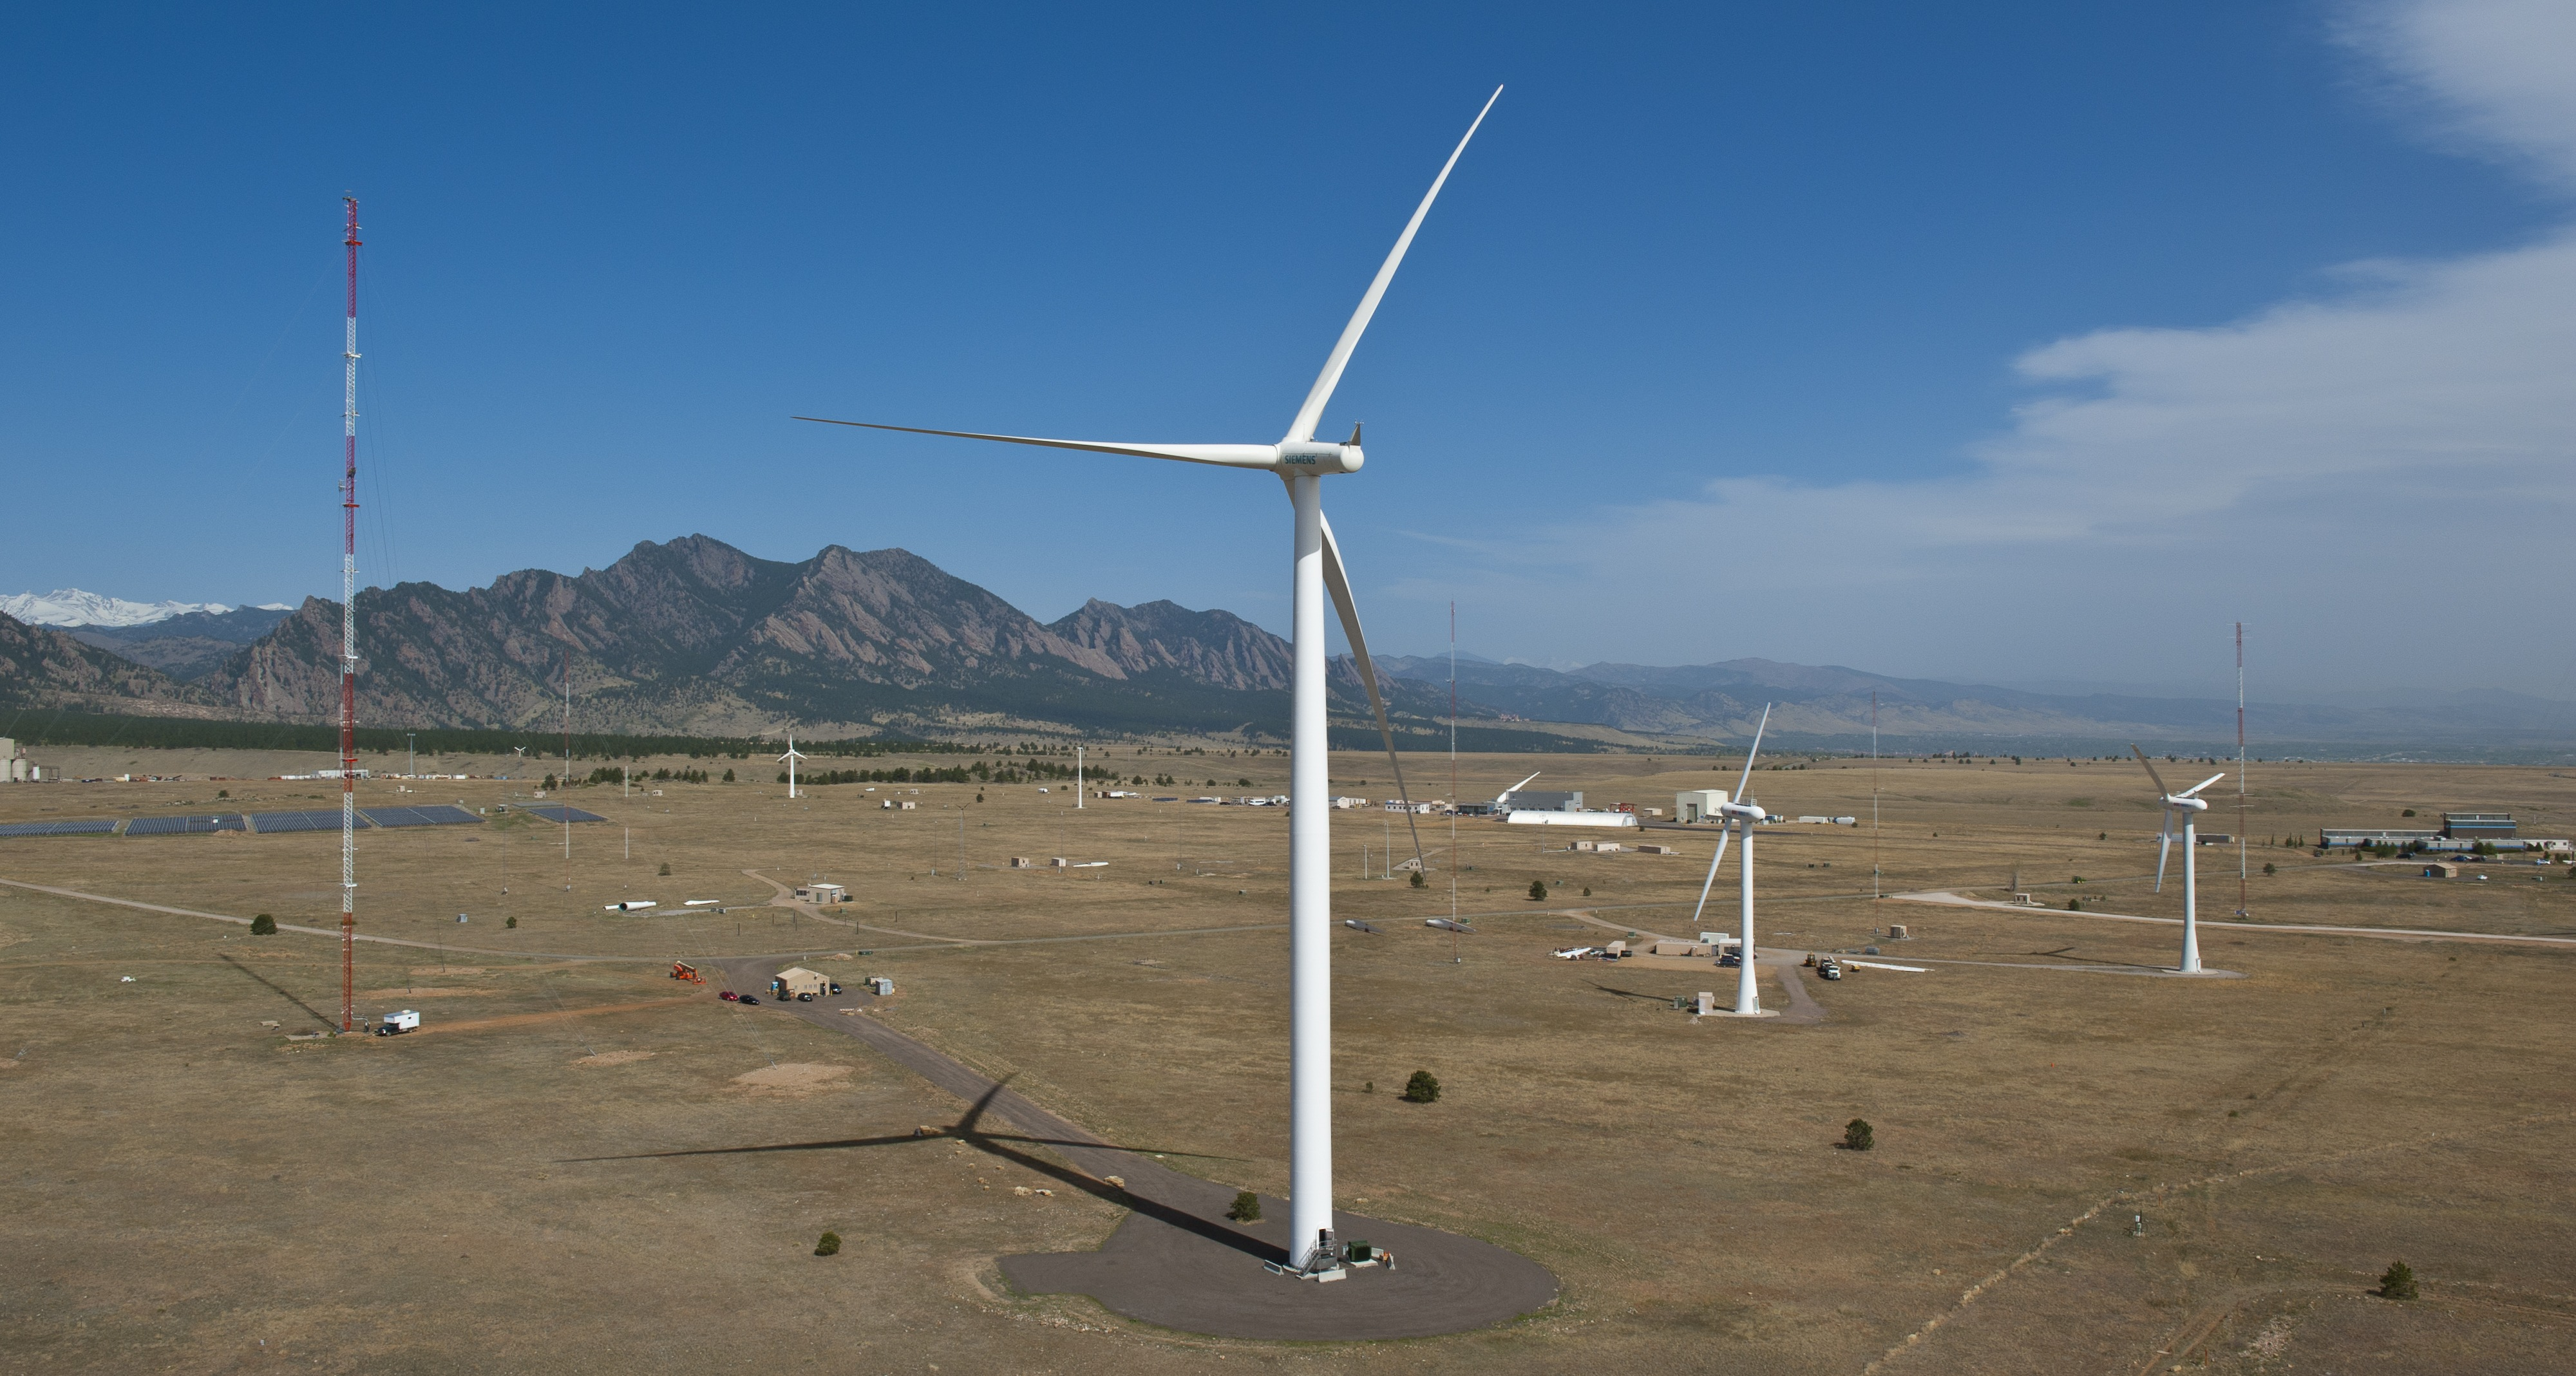
\includegraphics[height=2.5in]{files/20018}}
\hfill
\caption{NREL images}\label{fig:NRELimages}
\end{figure}
\end{verbatim}
 
\begin{figure*}[htp]
\centering
\hfill
\subfigure[Wind turbines at the Forward Wind Energy Center in Fond du Lac and Dodge Counties, Wisconsin. (Photo by Ruth Baranowski / NREL)\label{fig:21206}]{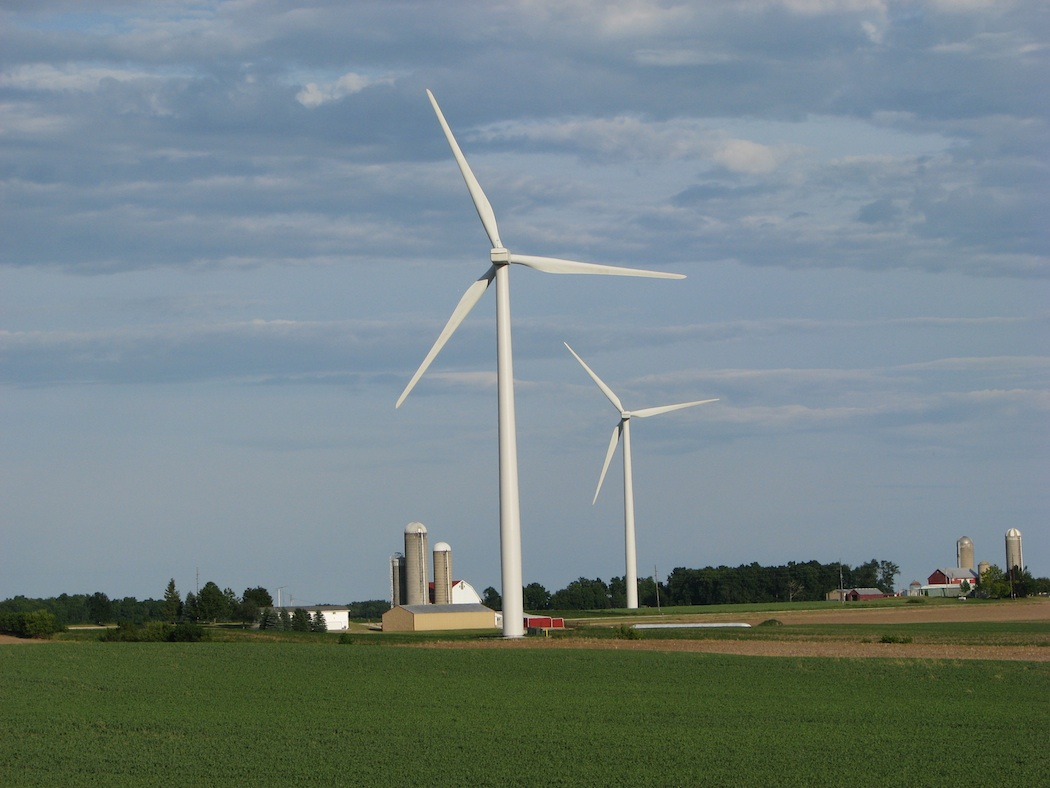
\includegraphics[height=2.5in]{files/21206}}
~ %add desired spacing between images, e. g. ~, \quad, \qquad etc. (or a blank line to force the subfigure onto a new line)
\hfill
\subfigure[Aerial view of the National Wind Technology Center. (Photo by Dennis Schroeder / NREL)\label{fig:20018}]{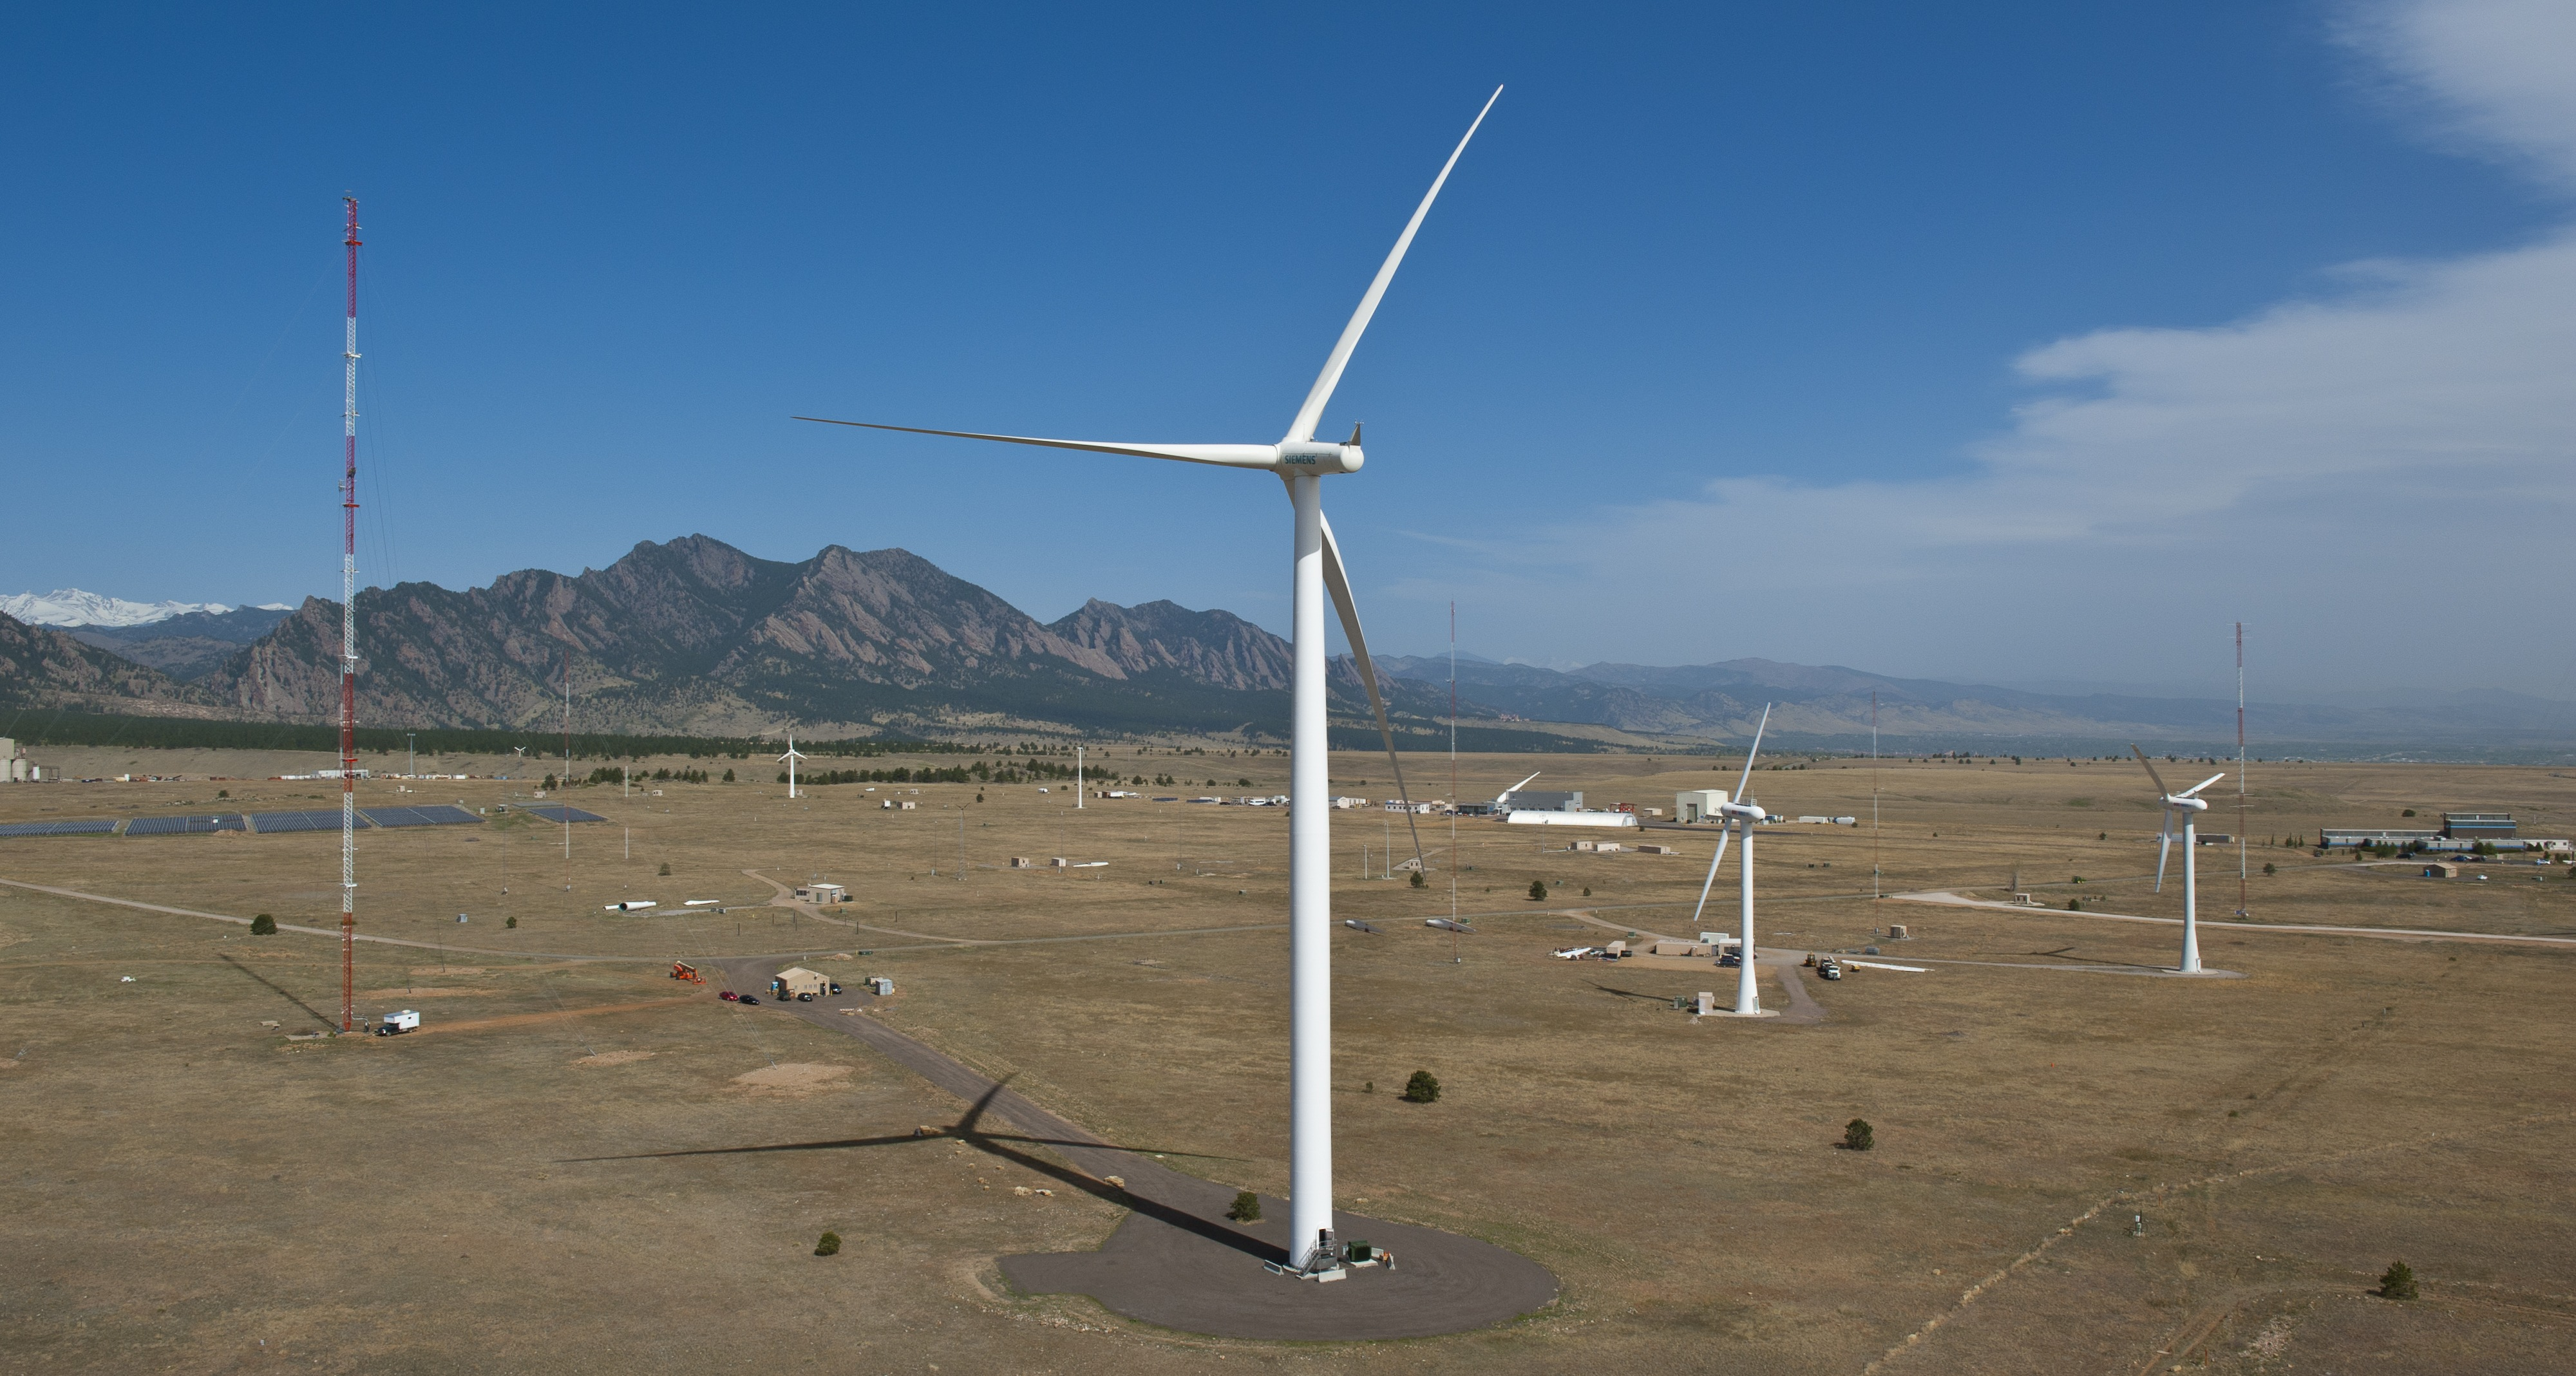
\includegraphics[height=2.5in]{files/20018}}
\hfill
\caption{NREL images}\label{fig:NRELimages}
\end{figure*}

If a subfigure is split over two lines using \verb+\\+, make sure those symbols are on their own line.

\section{Lists}

To make lists with automatic numbering, use the \texttt{enumerate} environment:

\begin{enumerate}
\item Like this,
\item and like this.
\end{enumerate}
\dots or bullet points \dots
\begin{itemize}
\item Like this,
\item and like this.
\end{itemize}

\section{Computer code}
The \texttt{lstlisting} package has been loaded.

\section{Creating a file structure}
\label{sec:FileStructure}
Use the \texttt{input} command to import other files into your main file. For example, each of the chapters in this report could be in separate files, called \emph{NRELRequirements} (Chapter 1), \emph{LatexAtNREL} (Chapter 2), and so-on. 

\begin{verbatim}
...
% content
\input{NRELRequirements}
\input{LatexAtNREL}
\input{LatexExamples}
\input{ConvertingToDoc}
...
\end{verbatim}

\input{ConvertingToDoc}
...
\end{verbatim}

\input{ConvertingToDoc}
...
\end{verbatim}

%% CHAPTER:MAKING DOC FILES
%\chapter{Preparing a .DOC or .DOCX file from LaTeX}\label{sec:latextodoc}
LaTeX users may find that they are required to convert their files into other formats for review or  editing. This section describes how LaTeX files can be converted into files that can be used with Microsoft Word.

\section{The conversion process} 
The NREL style has been designed to be converted into \emph{.doc} or \emph{.docx}. This can be achieved via one of two routes:
\begin{enumerate}
\item converting the latex file to rich text format (\emph{.rtf}) using \texttt{latex2rtf}, then importing the file into a word processor, or
\item converting the latex file to doc using pandoc.
\end{enumerate}

The performance of \texttt{Latex2rtf} and \texttt{pandoc} are compared in Table \ref{tab:conversioncomparison}.

\begin{table}[!h]
\centering
\caption{A comparison of latex2rtf and pandoc for document conversion.}\label{tab:conversioncomparison}
\begin{tabular}{lcc}
consideration & latex2rtf & pandoc \\\hline
requires changes to latex preamble & yes & no\\
output format & .rtf & .docx \\
supports cross references & yes & no\\
supports subfigures & partially & no\\
\end{tabular}
\end{table}

At this time, \texttt{latex2rtf} is the recommended tool for converting LaTeX files that have been made with the NREL class file, into word processor-readable files.

\section{Using latex2rtf to convert files}
The \texttt{latex2rtf} program reads LaTeX files and converts common LaTeX commands into their RTF equivalent. It is effectively another LaTeX interpreter that knows a limited subset of LaTeX. See the documentation at \href{http://sourceforge.net/projects/latex2rtf/}{http://sourceforge.net/projects/latex2rtf/} for details.

\subsection{Using latex2rtf}
To convert a document from LaTeX to RTF, follow these steps:
\begin{enumerate}
\item Install \texttt{latex2rtf}
\item Compile the document in LaTeX using the NREL class with the \texttt{book,report}, or \texttt{article} option, remembering to update the bibliography and cross references. The sequence of commands is:
\item Convert the document to RTF format using \texttt{latex2rtf}. The example .rtf file included with this document is created as follows:
\begin{verbatim}
latex2rtf -o latex2rtf_demo.rtf -f3 intro_to_NREL_latex
\end{verbatim}
\item Open the RTF file in Microsoft Word.
\item If the document contains tables of contents, tables of figures, tables of tables, or cross-references, select that text and update the fields.
\item Save the RTF file as a word-format document.
\end{enumerate}

\subsection{Using latex2rtf and LaTeX together}
Because \texttt{latex2rtf} only knows a subset of LaTeX, it is important to account for this when preparing a LaTeX document. The biggest problem is the lack of many packages, which is why authors are encouraged to use the NREL class file, which is known to work well with \texttt{latex2rtf}. Sometimes, though, it is important to be able to remove formatting for compatibility with \texttt{latex2rtf}, and so the preamble to this document includes a check to see if \texttt{latex2rtf} is being used:

\begin{verbatim}
\newif\iflatextortf
\iflatextortf
	\documentclass[12pt,letterpaper]{report}
	% File NRELLatex2rtf.tex

% set margins
\usepackage[margin=1 in,letterpaper]{geometry}

% use citations
\usepackage[sort]{natbib}

% change the heading of the bibliography
\renewcommand{\bibsection}{\section{References}}

% redefine \pdftooltip so that it behaves differently with and without latextortf
\newcommand{\pdftooltip}[3][]{#2}

%redefine the checkmark
\newcommand{\checkmark}{y\relax}

% redefine booktabs commands
\newcommand{\toprule}{\hline}
\newcommand{\midrule}{\hline}
\newcommand{\bottomrule}{\hline}

% redefine \href
\newcommand{\href}[2]{#1~ (\url{#2})}

% redefine \subfloat to match the \subfigure environment
\usepackage{subfigure}
\makeatletter
\newcommand{\subfloat}[2][]{\subfigure{\textit{Subcaption: \protect{#1}}}{#2}}
%\newcommand{\subfloat}[3][]{\subfigure{#1}{#2}{#3}}
% note that we can only have one '\label' in a figure environment
\makeatother

\newcommand{\subref}[1][]{\ref{#1}}

% redefine \todo so that it gives something useful
\newcommand{\todo}[2][]{\textbf{To Do:}~#2}

% deal with index entries:
\newcommand{\index}[1]{}
\else
	\documentclass[report]{nrel} 
\fi
\end{verbatim}

If \texttt{latex2rtf} is used, the boolean, \texttt{\textbackslash iflatextortf} will be TRUE and the commands will be interpreted as follows.
\begin{enumerate}
\item Set the document class to a generic LaTeX{} \emph{article}, \emph{report}, or \emph{book}. 
\item The file \emph{NRELLatex2rtf.tex} will be called, which maps most of the commands that are enabled in \emph{nrel.cls} to simpler versions that can be processed using \texttt{latex2rtf} (see Table \ref{Tab:Packages}).
\end{enumerate}

Authors that use packages other than those listed in Table \ref{Tab:Packages} may need to adjust the content of \emph{NRELLatex2rtf.tex} according to their needs. 

\subsection{Indexes}
Index entries will not be correctly converted to an \emph{.rtf} file. \emph{NRELLatex2rtf.tex} redefines the \verb+index+ command to do nothing when creating an \emph{.rtf} file. 

\subsection{What to do when the conversion to rich text format fails}
It is more than likely that the conversion to an \emph{.rtf} file will fail at some point. There are a few ways to deal with this:

\begin{description}
\item[Convert early and often.] Check that the document converts using \texttt{latex2rtf} every time a new environment is added.
\item[Try section-by-section.] Comment out the majority of the document and try to compile bit-by-bit. This will let you localize the error.
\item[Check new packages.] Please avoid using new packages. If a package has to be used, try the conversion immediately. If \texttt{latex2rtf} doesn't support the package, edit the file \emph{NRELLatex2rtf.tex} to redefine those commands to something that will convert appropriately. Put \emph{NRELLatex2rtf.tex} in the same directory as the LaTeX file to be converted.
\item[Avoid custom commands.] \texttt{latex2rtf} sometimes chokes on custom commands. A list of all recognized commands is available in the manual at \href{http://latex2rtf.sourceforge.net/latex2rtf.pdf}{http://latex2rtf.sourceforge.net/latex2rtf.pdf}. If custom commands are used, they may need to be redefined to work with the commands that \texttt{latex2rtf} does recognize. This can also be done in \emph{NRELLatex2rtf.tex}. You can check macros using the flag \verb+-d2+ when running \texttt{latex2rtf}.
\item[Use copy-paste.] Compile the whole document as a PDF, and save it somewhere. Then recompile using the reduced document that works with \texttt{latex2rtf}. Edit this in word and copy in the bits that killed the conversion.
\item[Talk to a communications rep.] If a document cannot be produced any other way than LaTeX with lots of packages, and \texttt{latex2rtf} just refuses to process it into a rich text file, discuss the process for having the PDF processed.
\end{description}

\section{Using pandoc}
Pandoc is a tool for converting documents between different formats. Pandoc is available at \href{http://johnmacfarlane.net/pandoc/}{http://johnmacfarlane.net/pandoc/}. Like \texttt{latex2rtf}, pandoc only supports a subset of latex commands and is not guaranteed to work for all applications.

Pandoc has several advantages over latex2rtf:
\begin{itemize}
\item Pandoc it supports conversion from latex to many other document formats (e.g. .html as well as .docx). However, there are other well-established tools to go directly from latex source code to other formats that may have better performance.
\item Pandoc does not require any changes to the latex source files.
\end{itemize}

To use pandoc, follow the installation instructions on the pandoc website, and then run pandoc from the command line. To convert this file, use the following command at the command line:

\begin{verbatim}
pandoc -o conversion_demo/pandoc_demo.docx intro_to_NREL_latex.tex --bibliography bibliography.bib --default-image-extension=.jpg
\end{verbatim}


%% CHAPTER: MAKING PDFS
\chapter{Preparing a high-quality PDF from LaTeX}\label{sec:PDFprep}
If the author chooses to complete the publications process using LaTeX\, the author must incorporate feedback and edits in to the LaTeX source files and prepare the final PDF, following these guidelines.

\section{PDF tagging}\label{sec:PDFtagging}
PDF tagging is a process whereby the components of the PDF document (headings, figures, tables, text) are marked so that a document reader can understand the document. This is useful when text to speech converters are being used. The process of tagging is also known as structuring, so that a tagged document might also be referred to as a structured document.

LaTeX does not prepare a tagged PDF document. The current solution to this is to use the tagging capability built in to Adobe's Acrobat Pro.

To prepare a tagged document, follow these steps:
\begin{enumerate}
\item Add tags. Go to the `Advanced' menu. Select `Accessibility', then `Add tags to document'.
\item Add alternative text for figures. Context-click the Figure, select `Properties', and fill in `Alternate Text'. Alternatively, try the process outlined below.
\item Specify the document language. Go to the `File' menu. Select `Document Properties', then the `Advanced' tab, `Language' field. In some versions of Acrobat, the sequence is `File', `Properties', `Reading Options', `Language'.
\item Define tab order.
\begin{enumerate}
\item Go to the `View' menu. Select `Navigation tabs', then `Pages'.
\item Click on any page, then type Ctrl-A (or Command-A on a Mac) to select all the pages.
\item Go to the `Options' menu in the top right of the dialog box, and select `Page Properties'
\item In the `Tab Order' tab, select `Use document structure'.
\end{enumerate}
\item Make sure tables have headings. 
\begin{enumerate}
\item Go to the `View' menu. Select `Navigation tabs', then `Tags'.
\item Select the `Tags' tab. This panel shows the document structure as a tree.
\item Navigate to the table cells that should be headers.
\item Check they have the type <TH>. If not, then right click on the header cell, select `properties', select the `Tag' tab, and change the value for `Type' to <TH>.
\end{enumerate}
\item Make sure all Chapters (or sections, if there are no chapters in the document) are correctly tagged.
\end{enumerate}

\section{Alt-text on images and equations}
`Alt text' is a textual description of an equation, link or figure. The following short equation should pop-up some text when a user passes a mouse over it. This should work in most PDF readers:
\begin{equation}
\pdftooltip{a^2+b^2=c^2}{An equation}
%a^2+b^2=c^2
\end{equation}

The alt text can be added after the PDF is compiled, or written in to the source document. The rest of this section describes how it can be added to the source and generated by LaTeX using the \href{pdfcomment}{http://www.ctan.org/pkg/pdfcomment} package. The general form of the command is:

\begin{verbatim}
\pdftooltip{<item>}{<pop-up text>}
\end{verbatim}

The previous equation was generated using this code:

\begin{verbatim}
\begin{equation}
\pdftooltip{a^2+b^2=c^2}{An equation}
\end{equation}
\end{verbatim}

The same approach can be used to create alt-text for images. For example, Figure \ref{fig:NRELimagesWithAltText} has been labeled. The code for this image is:

\begin{verbatim}
\begin{figure}[!h]
\centering
\hfill
\subfigure[Wind turbines at the Forward Wind Energy Center in Fond du Lac and Dodge Counties, Wisconsin. (Photo by Ruth Baranowski / NREL)] {\pdftooltip{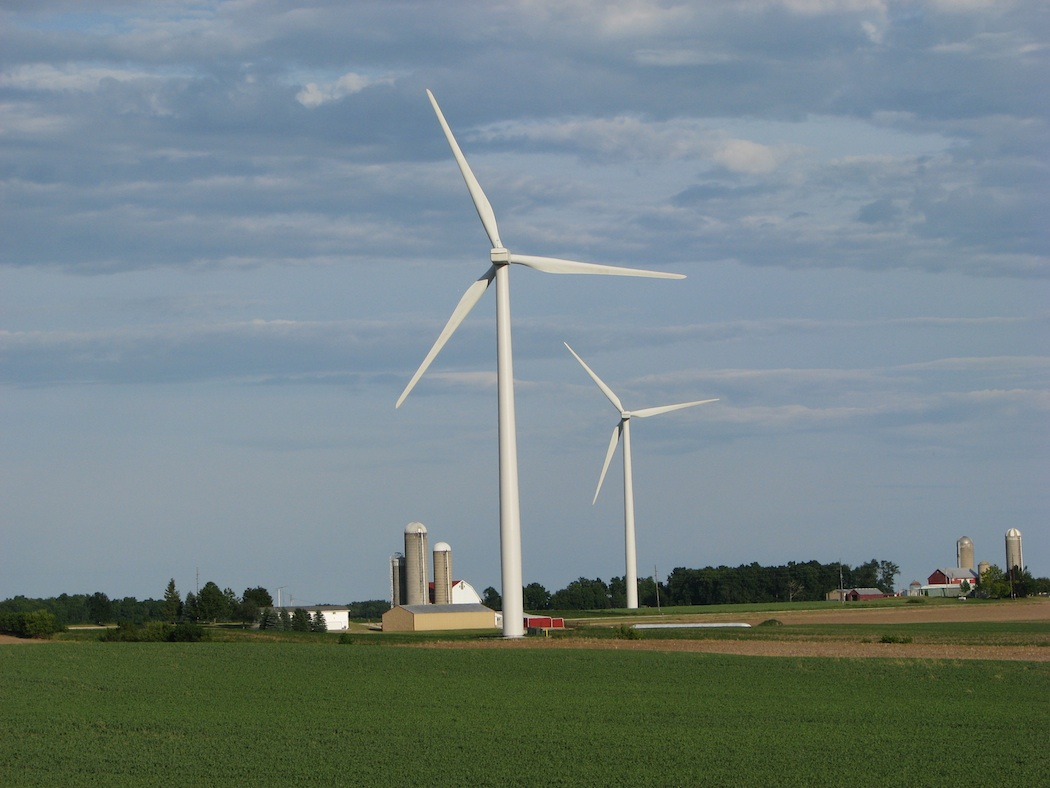
\includegraphics[height=2.5in]{files/21206}}{This is an image}}
~ 
\hfill
\subfigure[Aerial view of the National Wind Technology Center.  (Photo by Dennis Schroeder / NREL)] {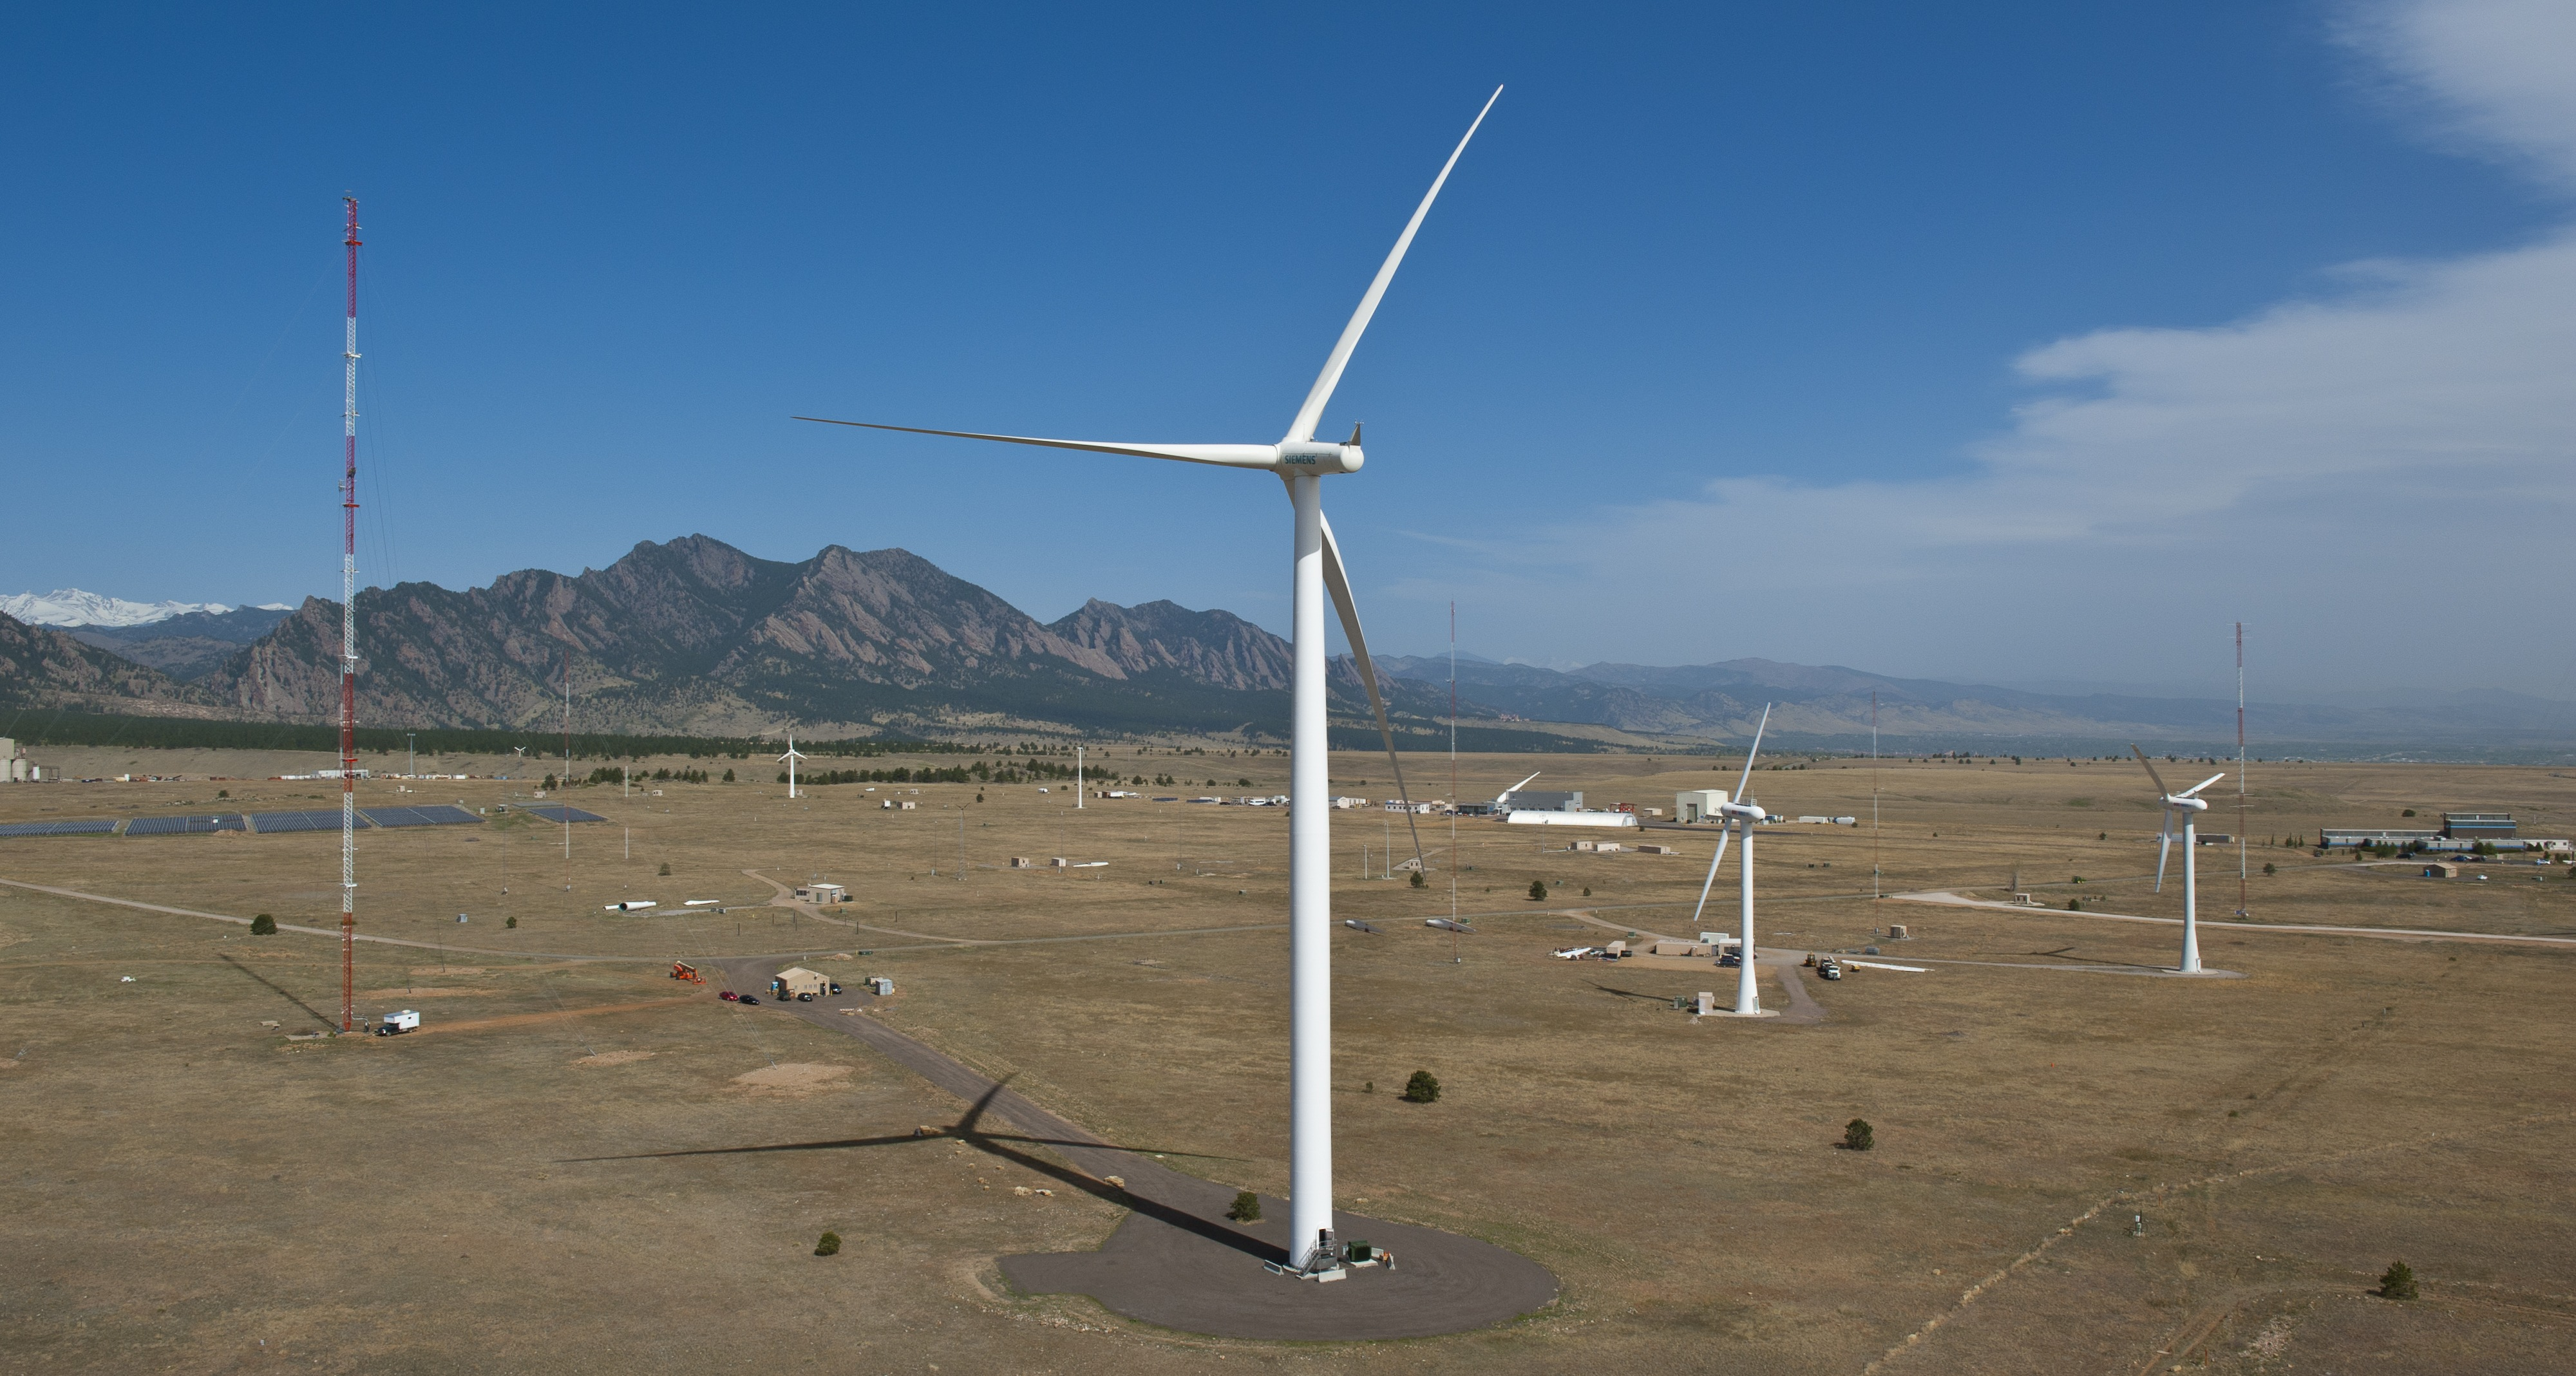
\includegraphics[height=2.5in]{files/20018}}
\hfill
\caption{NREL images}\label{fig:NRELimagesWithAltText}
\end{figure}
\end{verbatim}

\begin{figure}[!h]
\centering
\hfill
\subfigure[Wind turbines at the Forward Wind Energy Center in Fond du Lac and Dodge Counties, Wisconsin. (Photo by Ruth Baranowski / NREL)]{\pdftooltip{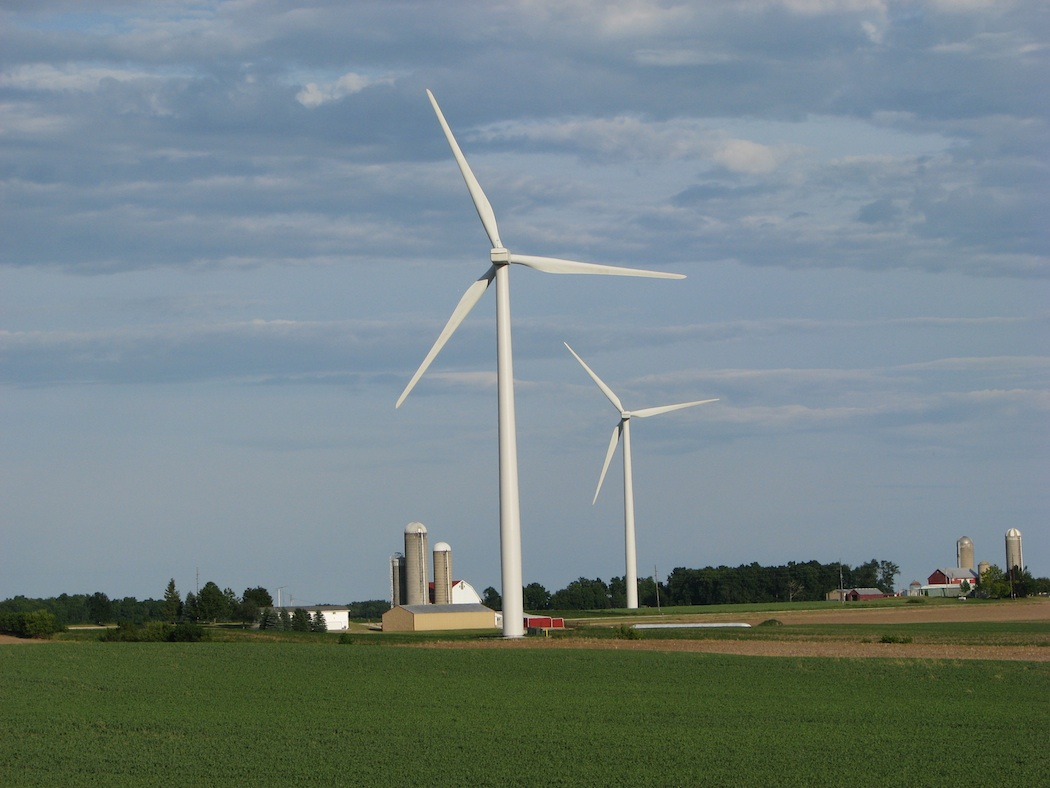
\includegraphics[height=2.5in]{files/21206}}{This is an image. It may be possible to propagate the caption into this text.}}
%{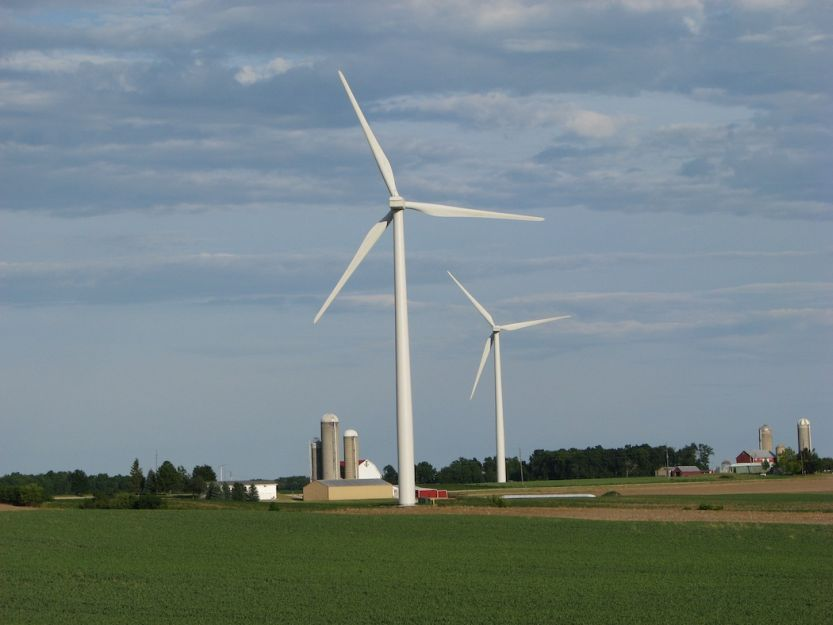
\includegraphics[height=2.5in]{21206}}
~ %add desired spacing between images, e. g. ~, \quad, \qquad etc. (or a blank line to force the subfigure onto a new line)
\hfill
\subfigure[Aerial view of the National Wind Technology Center. (Photo by Dennis Schroeder / NREL)]{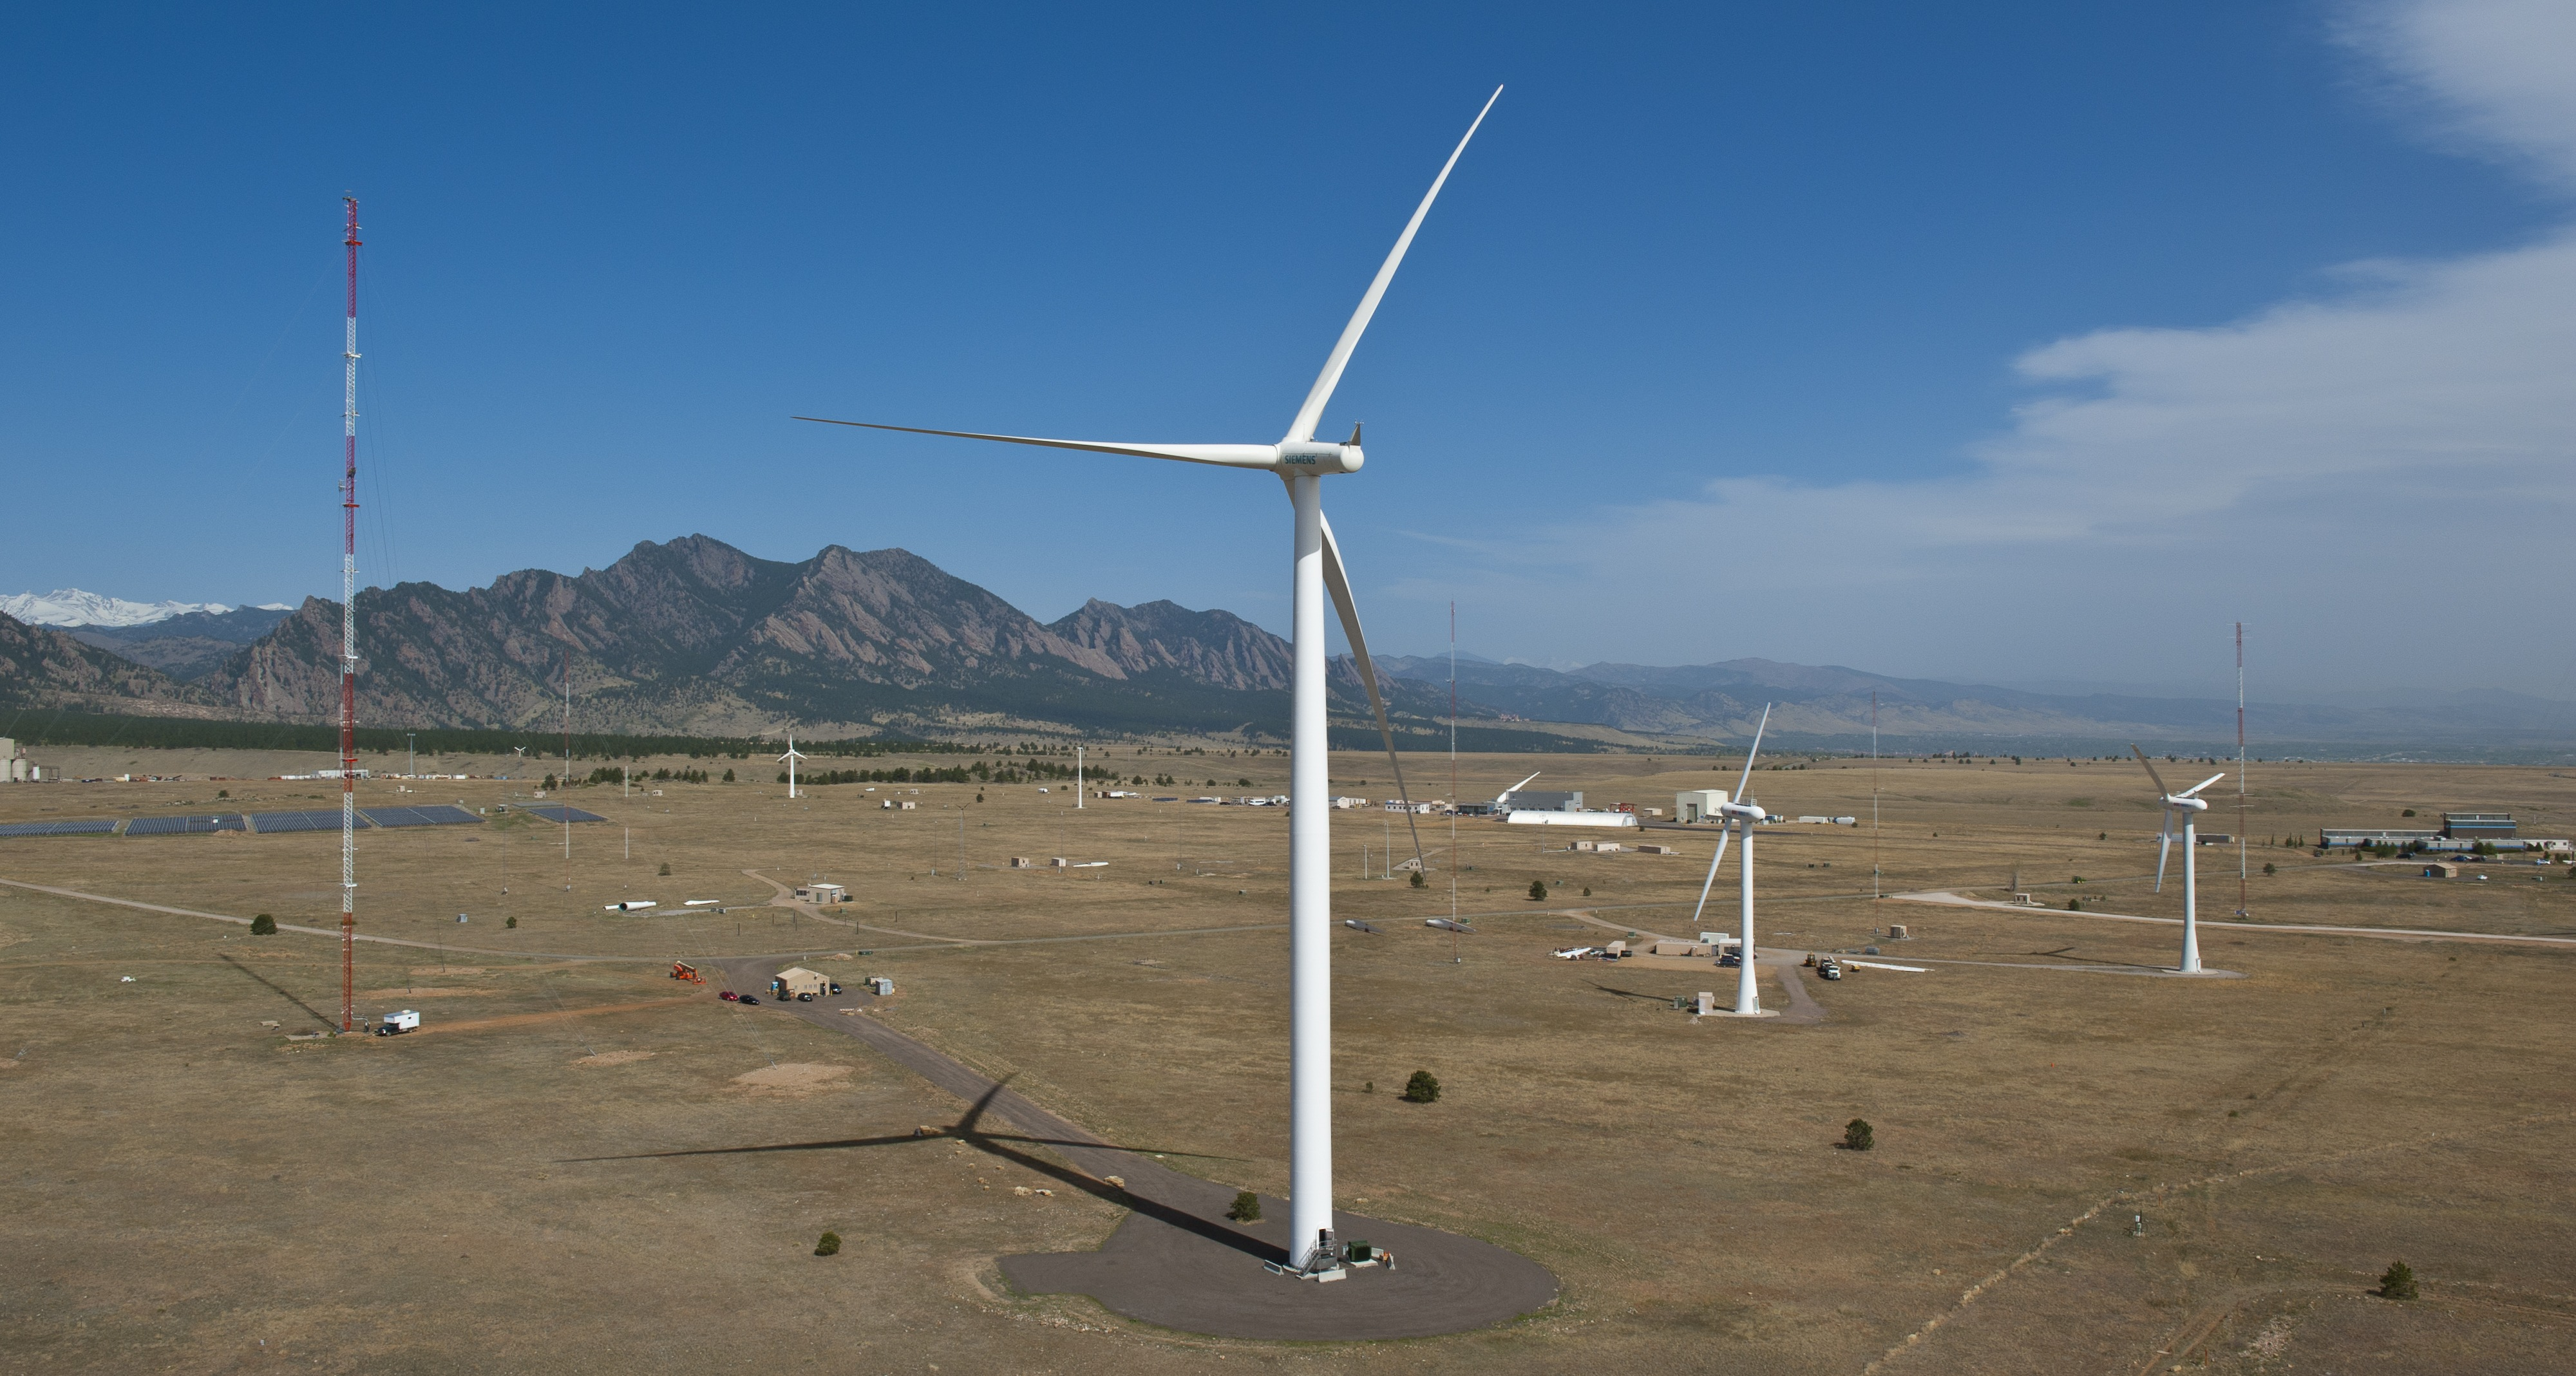
\includegraphics[height=2.5in]{files/20018}}
\hfill
\caption{NREL images}\label{fig:NRELimagesWithAltText}
\end{figure}

Alt-text is not processed by \texttt{latex2rtf}. So, if the author anticipates finishing the publication solely as a .DOC or .DOCX file, they do not need to use alt-text.

\section{Embedded fonts}
NREL requires that all fonts be embedded in the the final PDF. Check the PDF for embedded fonts using a PDF viewer. For example, in Adobe Acrobat Reader, look at the `fonts' tag of the document properties. If any fonts are not shown as being an \emph{embedded subset}, try the conversion again. 

Encapsulated postscript figures are particularly prone to having undefined fonts. Check by compiling the document in draft mode, and seeing if the fonts are still present in the output PDF. To fix this problem, consider changing the \emph{.eps} file to a \emph{.png}. To do this `on the fly', use this in the document's preamble:

\begin{verbatim}
\usepackage{epstopdf}
\epstopdfDeclareGraphicsRule
 {.eps}{png}{.png}{convert eps:\SourceFile.\SourceExt png:\OutputFile}
\AppendGraphicsExtensions{.png}
\end{verbatim}

% bibliography
\cleardoublepage
\label{sec:Bib}
\printbibliography
\end{document}